
% Default to the notebook output style

    


% Inherit from the specified cell style.




    
\documentclass[11pt]{article}

    
    
    \usepackage[T1]{fontenc}
    % Nicer default font (+ math font) than Computer Modern for most use cases
    \usepackage{mathpazo}

    % Basic figure setup, for now with no caption control since it's done
    % automatically by Pandoc (which extracts ![](path) syntax from Markdown).
    \usepackage{graphicx}
    % We will generate all images so they have a width \maxwidth. This means
    % that they will get their normal width if they fit onto the page, but
    % are scaled down if they would overflow the margins.
    \makeatletter
    \def\maxwidth{\ifdim\Gin@nat@width>\linewidth\linewidth
    \else\Gin@nat@width\fi}
    \makeatother
    \let\Oldincludegraphics\includegraphics
    % Set max figure width to be 80% of text width, for now hardcoded.
    \renewcommand{\includegraphics}[1]{\Oldincludegraphics[width=.8\maxwidth]{#1}}
    % Ensure that by default, figures have no caption (until we provide a
    % proper Figure object with a Caption API and a way to capture that
    % in the conversion process - todo).
    \usepackage{caption}
    \DeclareCaptionLabelFormat{nolabel}{}
    \captionsetup{labelformat=nolabel}

    \usepackage{adjustbox} % Used to constrain images to a maximum size 
    \usepackage{xcolor} % Allow colors to be defined
    \usepackage{enumerate} % Needed for markdown enumerations to work
    \usepackage{geometry} % Used to adjust the document margins
    \usepackage{amsmath} % Equations
    \usepackage{amssymb} % Equations
    \usepackage{textcomp} % defines textquotesingle
    % Hack from http://tex.stackexchange.com/a/47451/13684:
    \AtBeginDocument{%
        \def\PYZsq{\textquotesingle}% Upright quotes in Pygmentized code
    }
    \usepackage{upquote} % Upright quotes for verbatim code
    \usepackage{eurosym} % defines \euro
    \usepackage[mathletters]{ucs} % Extended unicode (utf-8) support
    \usepackage[utf8x]{inputenc} % Allow utf-8 characters in the tex document
    \usepackage{fancyvrb} % verbatim replacement that allows latex
    \usepackage{grffile} % extends the file name processing of package graphics 
                         % to support a larger range 
    % The hyperref package gives us a pdf with properly built
    % internal navigation ('pdf bookmarks' for the table of contents,
    % internal cross-reference links, web links for URLs, etc.)
    \usepackage{hyperref}
    \usepackage{longtable} % longtable support required by pandoc >1.10
    \usepackage{booktabs}  % table support for pandoc > 1.12.2
    \usepackage[inline]{enumitem} % IRkernel/repr support (it uses the enumerate* environment)
    \usepackage[normalem]{ulem} % ulem is needed to support strikethroughs (\sout)
                                % normalem makes italics be italics, not underlines
    

    
    
    % Colors for the hyperref package
    \definecolor{urlcolor}{rgb}{0,.145,.698}
    \definecolor{linkcolor}{rgb}{.71,0.21,0.01}
    \definecolor{citecolor}{rgb}{.12,.54,.11}

    % ANSI colors
    \definecolor{ansi-black}{HTML}{3E424D}
    \definecolor{ansi-black-intense}{HTML}{282C36}
    \definecolor{ansi-red}{HTML}{E75C58}
    \definecolor{ansi-red-intense}{HTML}{B22B31}
    \definecolor{ansi-green}{HTML}{00A250}
    \definecolor{ansi-green-intense}{HTML}{007427}
    \definecolor{ansi-yellow}{HTML}{DDB62B}
    \definecolor{ansi-yellow-intense}{HTML}{B27D12}
    \definecolor{ansi-blue}{HTML}{208FFB}
    \definecolor{ansi-blue-intense}{HTML}{0065CA}
    \definecolor{ansi-magenta}{HTML}{D160C4}
    \definecolor{ansi-magenta-intense}{HTML}{A03196}
    \definecolor{ansi-cyan}{HTML}{60C6C8}
    \definecolor{ansi-cyan-intense}{HTML}{258F8F}
    \definecolor{ansi-white}{HTML}{C5C1B4}
    \definecolor{ansi-white-intense}{HTML}{A1A6B2}

    % commands and environments needed by pandoc snippets
    % extracted from the output of `pandoc -s`
    \providecommand{\tightlist}{%
      \setlength{\itemsep}{0pt}\setlength{\parskip}{0pt}}
    \DefineVerbatimEnvironment{Highlighting}{Verbatim}{commandchars=\\\{\}}
    % Add ',fontsize=\small' for more characters per line
    \newenvironment{Shaded}{}{}
    \newcommand{\KeywordTok}[1]{\textcolor[rgb]{0.00,0.44,0.13}{\textbf{{#1}}}}
    \newcommand{\DataTypeTok}[1]{\textcolor[rgb]{0.56,0.13,0.00}{{#1}}}
    \newcommand{\DecValTok}[1]{\textcolor[rgb]{0.25,0.63,0.44}{{#1}}}
    \newcommand{\BaseNTok}[1]{\textcolor[rgb]{0.25,0.63,0.44}{{#1}}}
    \newcommand{\FloatTok}[1]{\textcolor[rgb]{0.25,0.63,0.44}{{#1}}}
    \newcommand{\CharTok}[1]{\textcolor[rgb]{0.25,0.44,0.63}{{#1}}}
    \newcommand{\StringTok}[1]{\textcolor[rgb]{0.25,0.44,0.63}{{#1}}}
    \newcommand{\CommentTok}[1]{\textcolor[rgb]{0.38,0.63,0.69}{\textit{{#1}}}}
    \newcommand{\OtherTok}[1]{\textcolor[rgb]{0.00,0.44,0.13}{{#1}}}
    \newcommand{\AlertTok}[1]{\textcolor[rgb]{1.00,0.00,0.00}{\textbf{{#1}}}}
    \newcommand{\FunctionTok}[1]{\textcolor[rgb]{0.02,0.16,0.49}{{#1}}}
    \newcommand{\RegionMarkerTok}[1]{{#1}}
    \newcommand{\ErrorTok}[1]{\textcolor[rgb]{1.00,0.00,0.00}{\textbf{{#1}}}}
    \newcommand{\NormalTok}[1]{{#1}}
    
    % Additional commands for more recent versions of Pandoc
    \newcommand{\ConstantTok}[1]{\textcolor[rgb]{0.53,0.00,0.00}{{#1}}}
    \newcommand{\SpecialCharTok}[1]{\textcolor[rgb]{0.25,0.44,0.63}{{#1}}}
    \newcommand{\VerbatimStringTok}[1]{\textcolor[rgb]{0.25,0.44,0.63}{{#1}}}
    \newcommand{\SpecialStringTok}[1]{\textcolor[rgb]{0.73,0.40,0.53}{{#1}}}
    \newcommand{\ImportTok}[1]{{#1}}
    \newcommand{\DocumentationTok}[1]{\textcolor[rgb]{0.73,0.13,0.13}{\textit{{#1}}}}
    \newcommand{\AnnotationTok}[1]{\textcolor[rgb]{0.38,0.63,0.69}{\textbf{\textit{{#1}}}}}
    \newcommand{\CommentVarTok}[1]{\textcolor[rgb]{0.38,0.63,0.69}{\textbf{\textit{{#1}}}}}
    \newcommand{\VariableTok}[1]{\textcolor[rgb]{0.10,0.09,0.49}{{#1}}}
    \newcommand{\ControlFlowTok}[1]{\textcolor[rgb]{0.00,0.44,0.13}{\textbf{{#1}}}}
    \newcommand{\OperatorTok}[1]{\textcolor[rgb]{0.40,0.40,0.40}{{#1}}}
    \newcommand{\BuiltInTok}[1]{{#1}}
    \newcommand{\ExtensionTok}[1]{{#1}}
    \newcommand{\PreprocessorTok}[1]{\textcolor[rgb]{0.74,0.48,0.00}{{#1}}}
    \newcommand{\AttributeTok}[1]{\textcolor[rgb]{0.49,0.56,0.16}{{#1}}}
    \newcommand{\InformationTok}[1]{\textcolor[rgb]{0.38,0.63,0.69}{\textbf{\textit{{#1}}}}}
    \newcommand{\WarningTok}[1]{\textcolor[rgb]{0.38,0.63,0.69}{\textbf{\textit{{#1}}}}}
    
    
    % Define a nice break command that doesn't care if a line doesn't already
    % exist.
    \def\br{\hspace*{\fill} \\* }
    % Math Jax compatability definitions
    \def\gt{>}
    \def\lt{<}
    % Document parameters
    \title{Neural Network}
    
    
    

    % Pygments definitions
    
\makeatletter
\def\PY@reset{\let\PY@it=\relax \let\PY@bf=\relax%
    \let\PY@ul=\relax \let\PY@tc=\relax%
    \let\PY@bc=\relax \let\PY@ff=\relax}
\def\PY@tok#1{\csname PY@tok@#1\endcsname}
\def\PY@toks#1+{\ifx\relax#1\empty\else%
    \PY@tok{#1}\expandafter\PY@toks\fi}
\def\PY@do#1{\PY@bc{\PY@tc{\PY@ul{%
    \PY@it{\PY@bf{\PY@ff{#1}}}}}}}
\def\PY#1#2{\PY@reset\PY@toks#1+\relax+\PY@do{#2}}

\expandafter\def\csname PY@tok@gd\endcsname{\def\PY@tc##1{\textcolor[rgb]{0.63,0.00,0.00}{##1}}}
\expandafter\def\csname PY@tok@gu\endcsname{\let\PY@bf=\textbf\def\PY@tc##1{\textcolor[rgb]{0.50,0.00,0.50}{##1}}}
\expandafter\def\csname PY@tok@gt\endcsname{\def\PY@tc##1{\textcolor[rgb]{0.00,0.27,0.87}{##1}}}
\expandafter\def\csname PY@tok@gs\endcsname{\let\PY@bf=\textbf}
\expandafter\def\csname PY@tok@gr\endcsname{\def\PY@tc##1{\textcolor[rgb]{1.00,0.00,0.00}{##1}}}
\expandafter\def\csname PY@tok@cm\endcsname{\let\PY@it=\textit\def\PY@tc##1{\textcolor[rgb]{0.25,0.50,0.50}{##1}}}
\expandafter\def\csname PY@tok@vg\endcsname{\def\PY@tc##1{\textcolor[rgb]{0.10,0.09,0.49}{##1}}}
\expandafter\def\csname PY@tok@vi\endcsname{\def\PY@tc##1{\textcolor[rgb]{0.10,0.09,0.49}{##1}}}
\expandafter\def\csname PY@tok@vm\endcsname{\def\PY@tc##1{\textcolor[rgb]{0.10,0.09,0.49}{##1}}}
\expandafter\def\csname PY@tok@mh\endcsname{\def\PY@tc##1{\textcolor[rgb]{0.40,0.40,0.40}{##1}}}
\expandafter\def\csname PY@tok@cs\endcsname{\let\PY@it=\textit\def\PY@tc##1{\textcolor[rgb]{0.25,0.50,0.50}{##1}}}
\expandafter\def\csname PY@tok@ge\endcsname{\let\PY@it=\textit}
\expandafter\def\csname PY@tok@vc\endcsname{\def\PY@tc##1{\textcolor[rgb]{0.10,0.09,0.49}{##1}}}
\expandafter\def\csname PY@tok@il\endcsname{\def\PY@tc##1{\textcolor[rgb]{0.40,0.40,0.40}{##1}}}
\expandafter\def\csname PY@tok@go\endcsname{\def\PY@tc##1{\textcolor[rgb]{0.53,0.53,0.53}{##1}}}
\expandafter\def\csname PY@tok@cp\endcsname{\def\PY@tc##1{\textcolor[rgb]{0.74,0.48,0.00}{##1}}}
\expandafter\def\csname PY@tok@gi\endcsname{\def\PY@tc##1{\textcolor[rgb]{0.00,0.63,0.00}{##1}}}
\expandafter\def\csname PY@tok@gh\endcsname{\let\PY@bf=\textbf\def\PY@tc##1{\textcolor[rgb]{0.00,0.00,0.50}{##1}}}
\expandafter\def\csname PY@tok@ni\endcsname{\let\PY@bf=\textbf\def\PY@tc##1{\textcolor[rgb]{0.60,0.60,0.60}{##1}}}
\expandafter\def\csname PY@tok@nl\endcsname{\def\PY@tc##1{\textcolor[rgb]{0.63,0.63,0.00}{##1}}}
\expandafter\def\csname PY@tok@nn\endcsname{\let\PY@bf=\textbf\def\PY@tc##1{\textcolor[rgb]{0.00,0.00,1.00}{##1}}}
\expandafter\def\csname PY@tok@no\endcsname{\def\PY@tc##1{\textcolor[rgb]{0.53,0.00,0.00}{##1}}}
\expandafter\def\csname PY@tok@na\endcsname{\def\PY@tc##1{\textcolor[rgb]{0.49,0.56,0.16}{##1}}}
\expandafter\def\csname PY@tok@nb\endcsname{\def\PY@tc##1{\textcolor[rgb]{0.00,0.50,0.00}{##1}}}
\expandafter\def\csname PY@tok@nc\endcsname{\let\PY@bf=\textbf\def\PY@tc##1{\textcolor[rgb]{0.00,0.00,1.00}{##1}}}
\expandafter\def\csname PY@tok@nd\endcsname{\def\PY@tc##1{\textcolor[rgb]{0.67,0.13,1.00}{##1}}}
\expandafter\def\csname PY@tok@ne\endcsname{\let\PY@bf=\textbf\def\PY@tc##1{\textcolor[rgb]{0.82,0.25,0.23}{##1}}}
\expandafter\def\csname PY@tok@nf\endcsname{\def\PY@tc##1{\textcolor[rgb]{0.00,0.00,1.00}{##1}}}
\expandafter\def\csname PY@tok@si\endcsname{\let\PY@bf=\textbf\def\PY@tc##1{\textcolor[rgb]{0.73,0.40,0.53}{##1}}}
\expandafter\def\csname PY@tok@s2\endcsname{\def\PY@tc##1{\textcolor[rgb]{0.73,0.13,0.13}{##1}}}
\expandafter\def\csname PY@tok@nt\endcsname{\let\PY@bf=\textbf\def\PY@tc##1{\textcolor[rgb]{0.00,0.50,0.00}{##1}}}
\expandafter\def\csname PY@tok@nv\endcsname{\def\PY@tc##1{\textcolor[rgb]{0.10,0.09,0.49}{##1}}}
\expandafter\def\csname PY@tok@s1\endcsname{\def\PY@tc##1{\textcolor[rgb]{0.73,0.13,0.13}{##1}}}
\expandafter\def\csname PY@tok@dl\endcsname{\def\PY@tc##1{\textcolor[rgb]{0.73,0.13,0.13}{##1}}}
\expandafter\def\csname PY@tok@ch\endcsname{\let\PY@it=\textit\def\PY@tc##1{\textcolor[rgb]{0.25,0.50,0.50}{##1}}}
\expandafter\def\csname PY@tok@m\endcsname{\def\PY@tc##1{\textcolor[rgb]{0.40,0.40,0.40}{##1}}}
\expandafter\def\csname PY@tok@gp\endcsname{\let\PY@bf=\textbf\def\PY@tc##1{\textcolor[rgb]{0.00,0.00,0.50}{##1}}}
\expandafter\def\csname PY@tok@sh\endcsname{\def\PY@tc##1{\textcolor[rgb]{0.73,0.13,0.13}{##1}}}
\expandafter\def\csname PY@tok@ow\endcsname{\let\PY@bf=\textbf\def\PY@tc##1{\textcolor[rgb]{0.67,0.13,1.00}{##1}}}
\expandafter\def\csname PY@tok@sx\endcsname{\def\PY@tc##1{\textcolor[rgb]{0.00,0.50,0.00}{##1}}}
\expandafter\def\csname PY@tok@bp\endcsname{\def\PY@tc##1{\textcolor[rgb]{0.00,0.50,0.00}{##1}}}
\expandafter\def\csname PY@tok@c1\endcsname{\let\PY@it=\textit\def\PY@tc##1{\textcolor[rgb]{0.25,0.50,0.50}{##1}}}
\expandafter\def\csname PY@tok@fm\endcsname{\def\PY@tc##1{\textcolor[rgb]{0.00,0.00,1.00}{##1}}}
\expandafter\def\csname PY@tok@o\endcsname{\def\PY@tc##1{\textcolor[rgb]{0.40,0.40,0.40}{##1}}}
\expandafter\def\csname PY@tok@kc\endcsname{\let\PY@bf=\textbf\def\PY@tc##1{\textcolor[rgb]{0.00,0.50,0.00}{##1}}}
\expandafter\def\csname PY@tok@c\endcsname{\let\PY@it=\textit\def\PY@tc##1{\textcolor[rgb]{0.25,0.50,0.50}{##1}}}
\expandafter\def\csname PY@tok@mf\endcsname{\def\PY@tc##1{\textcolor[rgb]{0.40,0.40,0.40}{##1}}}
\expandafter\def\csname PY@tok@err\endcsname{\def\PY@bc##1{\setlength{\fboxsep}{0pt}\fcolorbox[rgb]{1.00,0.00,0.00}{1,1,1}{\strut ##1}}}
\expandafter\def\csname PY@tok@mb\endcsname{\def\PY@tc##1{\textcolor[rgb]{0.40,0.40,0.40}{##1}}}
\expandafter\def\csname PY@tok@ss\endcsname{\def\PY@tc##1{\textcolor[rgb]{0.10,0.09,0.49}{##1}}}
\expandafter\def\csname PY@tok@sr\endcsname{\def\PY@tc##1{\textcolor[rgb]{0.73,0.40,0.53}{##1}}}
\expandafter\def\csname PY@tok@mo\endcsname{\def\PY@tc##1{\textcolor[rgb]{0.40,0.40,0.40}{##1}}}
\expandafter\def\csname PY@tok@kd\endcsname{\let\PY@bf=\textbf\def\PY@tc##1{\textcolor[rgb]{0.00,0.50,0.00}{##1}}}
\expandafter\def\csname PY@tok@mi\endcsname{\def\PY@tc##1{\textcolor[rgb]{0.40,0.40,0.40}{##1}}}
\expandafter\def\csname PY@tok@kn\endcsname{\let\PY@bf=\textbf\def\PY@tc##1{\textcolor[rgb]{0.00,0.50,0.00}{##1}}}
\expandafter\def\csname PY@tok@cpf\endcsname{\let\PY@it=\textit\def\PY@tc##1{\textcolor[rgb]{0.25,0.50,0.50}{##1}}}
\expandafter\def\csname PY@tok@kr\endcsname{\let\PY@bf=\textbf\def\PY@tc##1{\textcolor[rgb]{0.00,0.50,0.00}{##1}}}
\expandafter\def\csname PY@tok@s\endcsname{\def\PY@tc##1{\textcolor[rgb]{0.73,0.13,0.13}{##1}}}
\expandafter\def\csname PY@tok@kp\endcsname{\def\PY@tc##1{\textcolor[rgb]{0.00,0.50,0.00}{##1}}}
\expandafter\def\csname PY@tok@w\endcsname{\def\PY@tc##1{\textcolor[rgb]{0.73,0.73,0.73}{##1}}}
\expandafter\def\csname PY@tok@kt\endcsname{\def\PY@tc##1{\textcolor[rgb]{0.69,0.00,0.25}{##1}}}
\expandafter\def\csname PY@tok@sc\endcsname{\def\PY@tc##1{\textcolor[rgb]{0.73,0.13,0.13}{##1}}}
\expandafter\def\csname PY@tok@sb\endcsname{\def\PY@tc##1{\textcolor[rgb]{0.73,0.13,0.13}{##1}}}
\expandafter\def\csname PY@tok@sa\endcsname{\def\PY@tc##1{\textcolor[rgb]{0.73,0.13,0.13}{##1}}}
\expandafter\def\csname PY@tok@k\endcsname{\let\PY@bf=\textbf\def\PY@tc##1{\textcolor[rgb]{0.00,0.50,0.00}{##1}}}
\expandafter\def\csname PY@tok@se\endcsname{\let\PY@bf=\textbf\def\PY@tc##1{\textcolor[rgb]{0.73,0.40,0.13}{##1}}}
\expandafter\def\csname PY@tok@sd\endcsname{\let\PY@it=\textit\def\PY@tc##1{\textcolor[rgb]{0.73,0.13,0.13}{##1}}}

\def\PYZbs{\char`\\}
\def\PYZus{\char`\_}
\def\PYZob{\char`\{}
\def\PYZcb{\char`\}}
\def\PYZca{\char`\^}
\def\PYZam{\char`\&}
\def\PYZlt{\char`\<}
\def\PYZgt{\char`\>}
\def\PYZsh{\char`\#}
\def\PYZpc{\char`\%}
\def\PYZdl{\char`\$}
\def\PYZhy{\char`\-}
\def\PYZsq{\char`\'}
\def\PYZdq{\char`\"}
\def\PYZti{\char`\~}
% for compatibility with earlier versions
\def\PYZat{@}
\def\PYZlb{[}
\def\PYZrb{]}
\makeatother


    % Exact colors from NB
    \definecolor{incolor}{rgb}{0.0, 0.0, 0.5}
    \definecolor{outcolor}{rgb}{0.545, 0.0, 0.0}



    
    % Prevent overflowing lines due to hard-to-break entities
    \sloppy 
    % Setup hyperref package
    \hypersetup{
      breaklinks=true,  % so long urls are correctly broken across lines
      colorlinks=true,
      urlcolor=urlcolor,
      linkcolor=linkcolor,
      citecolor=citecolor,
      }
    % Slightly bigger margins than the latex defaults
    
    \geometry{verbose,tmargin=1in,bmargin=1in,lmargin=1in,rmargin=1in}
    
    

    \begin{document}
    
    
    \maketitle
    
    

    
    ** Xiangyi Cheng (xxc273)**

    \hypertarget{concept-and-background}{%
\section{Concept and Background}\label{concept-and-background}}

    In this assignment, a baseline and a deep neural network are required to
be constructed. A dataset needs to be trained based on this neural
network. The performance trained from the baseline and the deep neural
network should be compared and discussed.

    A neural network is an artificial neural network with one or more hidden
layers between the input and output layers which is inspired by
biological neural networks that constitude animal brains. For the
simplest case that only one layer exists (the diagram is shown below).
Input is a set of observations, each an N-dimension vector. Weights are
assigned to generate the hidden layer from the input layer. After
obtaining the hidden layer, new weights are calculated to get the output
layer. Specifically saying, the hidden layer is made of nodes. A node
combines input from the data with a set of weights which called net
input function. Then the result is passed through a node called
activation function to determine if and how the signal progresses affect
the output. In this case, weights are fully connected which means each
node owns its weights from an input. 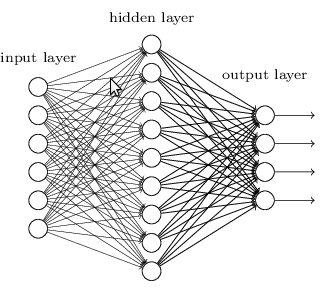
\includegraphics{nn.png}

Extend this basic idea to a deep neural network which includes multiple
layers. Once the first layer is obtained, the weights are assigned again
to generate a new layer. After several times, the network consists of
multiple layers which causes more accurate ultimate output. The diagram
below illuminates a three-hidden-layer neural network.
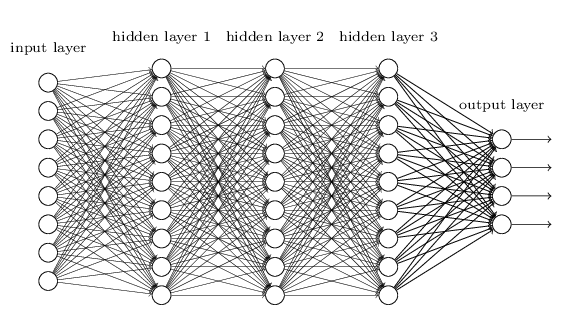
\includegraphics{dnn.png}

The weights mentioned above are the key to get a good model with
accurate predictions. Propper weights are obtained by ``back progagation
algorithm'' which was imbedded into many packages. And the common method
of optimization algorithm is ``gradient descent''. Applying this
algorithm, optimal weights are chosen to minimize the errors.

The applications of deep neural network are broad and play an important
role in several fields such as object detection and recognition,
automatic speech recognition, visual art processing, etc.. The packages
developed based on neural network are mature and various. In this
assignment, TensorFlow is used to construct a deep neural network and
train it on mnist dataset which is a large database of handwritten
digits included 60000 training images and 10000 test images. The
accuracy will be obtained after applying the training.

    \hypertarget{implement}{%
\section{Implement}\label{implement}}

    TensorFlow is an open-source software library used for machine learning
applications such as neural networks. Basically, we will use TensorFlow
to train the mnist database based on the models we build. The accuracy
will be computated and printed out. To achieve this goal, TensorFlow and
mnist database should be imported first.

    \begin{Verbatim}[commandchars=\\\{\}]
{\color{incolor}In [{\color{incolor}2}]:} \PY{k+kn}{import} \PY{n+nn}{tensorflow} \PY{k+kn}{as} \PY{n+nn}{tf}
        \PY{k+kn}{from} \PY{n+nn}{tensorflow.examples.tutorials.mnist} \PY{k+kn}{import} \PY{n}{input\PYZus{}data}
\end{Verbatim}


    Load the mnist and extract the data and label seperately. Class number
is 10 due to 10 digit numbers.

    \begin{Verbatim}[commandchars=\\\{\}]
{\color{incolor}In [{\color{incolor}3}]:} \PY{n}{mnist}\PY{o}{=}\PY{n}{input\PYZus{}data}\PY{o}{.}\PY{n}{read\PYZus{}data\PYZus{}sets}\PY{p}{(}\PY{l+s+s1}{\PYZsq{}}\PY{l+s+s1}{/tmp/data/}\PY{l+s+s1}{\PYZsq{}}\PY{p}{,}\PY{n}{one\PYZus{}hot}\PY{o}{=}\PY{n+nb+bp}{True}\PY{p}{)}
        
        
        \PY{n}{mnist\PYZus{}data}\PY{o}{=}\PY{n}{tf}\PY{o}{.}\PY{n}{placeholder}\PY{p}{(}\PY{l+s+s1}{\PYZsq{}}\PY{l+s+s1}{float}\PY{l+s+s1}{\PYZsq{}}\PY{p}{,}\PY{p}{[}\PY{n+nb+bp}{None}\PY{p}{,}\PY{l+m+mi}{784}\PY{p}{]}\PY{p}{)}
        \PY{n}{label}\PY{o}{=}\PY{n}{tf}\PY{o}{.}\PY{n}{placeholder}\PY{p}{(}\PY{l+s+s1}{\PYZsq{}}\PY{l+s+s1}{float}\PY{l+s+s1}{\PYZsq{}}\PY{p}{)}
        
        \PY{c+c1}{\PYZsh{} 10 different digit numbers: 0\PYZhy{}9}
        \PY{n}{n\PYZus{}classes}\PY{o}{=}\PY{l+m+mi}{10}
        \PY{n}{n\PYZus{}each\PYZus{}group}\PY{o}{=}\PY{l+m+mi}{100}
\end{Verbatim}


    \begin{Verbatim}[commandchars=\\\{\}]
Extracting /tmp/data/train-images-idx3-ubyte.gz
Extracting /tmp/data/train-labels-idx1-ubyte.gz
Extracting /tmp/data/t10k-images-idx3-ubyte.gz
Extracting /tmp/data/t10k-labels-idx1-ubyte.gz

    \end{Verbatim}

    \hypertarget{baseline-construction}{%
\subsection{Baseline Construction}\label{baseline-construction}}

A model include only one hidden layer is constructed. The compulational
idea is: \[ Hidden Layer = Input Data * weight + bias \]
\[ Output Layer = Hidden Layer * weight + bias \]

The nodes in hidden layer is set to 500 which could offer us a good
result without consuming heavy computations. The input value is 784
since each image in mnist is in 28*28 dimenions. An activation function
is called after obtaining the hidden layer.

    \begin{Verbatim}[commandchars=\\\{\}]
{\color{incolor}In [{\color{incolor}4}]:} \PY{k}{def} \PY{n+nf}{baseline\PYZus{}neural\PYZus{}network}\PY{p}{(}\PY{n}{data}\PY{p}{)}\PY{p}{:}
        	\PY{c+c1}{\PYZsh{} input\PYZus{}data * weight + bias}
        	\PY{c+c1}{\PYZsh{} the }
        	\PY{n}{n\PYZus{}hidden1}\PY{o}{=}\PY{l+m+mi}{500}
        
        	\PY{c+c1}{\PYZsh{} each image has 784 pixels which is calculated by 28*28.}
        	\PY{n}{hidden\PYZus{}layer1}\PY{o}{=}\PY{p}{\PYZob{}}\PY{l+s+s1}{\PYZsq{}}\PY{l+s+s1}{weights}\PY{l+s+s1}{\PYZsq{}}\PY{p}{:}\PY{n}{tf}\PY{o}{.}\PY{n}{Variable}\PY{p}{(}\PY{n}{tf}\PY{o}{.}\PY{n}{random\PYZus{}normal}\PY{p}{(}\PY{p}{[}\PY{l+m+mi}{784}\PY{p}{,}\PY{n}{n\PYZus{}hidden1}\PY{p}{]}\PY{p}{)}\PY{p}{)}\PY{p}{,}\PY{l+s+s1}{\PYZsq{}}\PY{l+s+s1}{biases}\PY{l+s+s1}{\PYZsq{}}\PY{p}{:}\PY{n}{tf}\PY{o}{.}\PY{n}{Variable}\PY{p}{(}\PY{n}{tf}\PY{o}{.}\PY{n}{random\PYZus{}normal}\PY{p}{(}\PY{p}{[}\PY{n}{n\PYZus{}hidden1}\PY{p}{]}\PY{p}{)}\PY{p}{)}\PY{p}{\PYZcb{}}
        
        	\PY{n}{output\PYZus{}layer}\PY{o}{=}\PY{p}{\PYZob{}}\PY{l+s+s1}{\PYZsq{}}\PY{l+s+s1}{weights}\PY{l+s+s1}{\PYZsq{}}\PY{p}{:}\PY{n}{tf}\PY{o}{.}\PY{n}{Variable}\PY{p}{(}\PY{n}{tf}\PY{o}{.}\PY{n}{random\PYZus{}normal}\PY{p}{(}\PY{p}{[}\PY{n}{n\PYZus{}hidden1}\PY{p}{,}\PY{n}{n\PYZus{}classes}\PY{p}{]}\PY{p}{)}\PY{p}{)}\PY{p}{,}\PY{l+s+s1}{\PYZsq{}}\PY{l+s+s1}{biases}\PY{l+s+s1}{\PYZsq{}}\PY{p}{:}\PY{n}{tf}\PY{o}{.}\PY{n}{Variable}\PY{p}{(}\PY{n}{tf}\PY{o}{.}\PY{n}{random\PYZus{}normal}\PY{p}{(}\PY{p}{[}\PY{n}{n\PYZus{}classes}\PY{p}{]}\PY{p}{)}\PY{p}{)}\PY{p}{\PYZcb{}}
        
        	\PY{n}{layer1} \PY{o}{=} \PY{n}{tf}\PY{o}{.}\PY{n}{add}\PY{p}{(}\PY{n}{tf}\PY{o}{.}\PY{n}{matmul}\PY{p}{(}\PY{n}{data}\PY{p}{,}\PY{n}{hidden\PYZus{}layer1}\PY{p}{[}\PY{l+s+s1}{\PYZsq{}}\PY{l+s+s1}{weights}\PY{l+s+s1}{\PYZsq{}}\PY{p}{]}\PY{p}{)}\PY{p}{,}\PY{n}{hidden\PYZus{}layer1}\PY{p}{[}\PY{l+s+s1}{\PYZsq{}}\PY{l+s+s1}{biases}\PY{l+s+s1}{\PYZsq{}}\PY{p}{]}\PY{p}{)}
        	\PY{n}{act\PYZus{}layer1} \PY{o}{=} \PY{n}{tf}\PY{o}{.}\PY{n}{nn}\PY{o}{.}\PY{n}{relu}\PY{p}{(}\PY{n}{layer1}\PY{p}{)}
        
        	\PY{n}{model} \PY{o}{=} \PY{n}{tf}\PY{o}{.}\PY{n}{matmul}\PY{p}{(}\PY{n}{act\PYZus{}layer1}\PY{p}{,}\PY{n}{output\PYZus{}layer}\PY{p}{[}\PY{l+s+s1}{\PYZsq{}}\PY{l+s+s1}{weights}\PY{l+s+s1}{\PYZsq{}}\PY{p}{]}\PY{p}{)}\PY{o}{+}\PY{n}{output\PYZus{}layer}\PY{p}{[}\PY{l+s+s1}{\PYZsq{}}\PY{l+s+s1}{biases}\PY{l+s+s1}{\PYZsq{}}\PY{p}{]}
        
        	\PY{k}{return} \PY{n}{model} 
\end{Verbatim}


    The training function is defined as below. The baseline neural network
model we built above is passed into the training function. In the code,
tf.train.AdamOptimizer().minimize() is applied to optimize the weights
by reducing the errors. To view the training process, 10 epoches should
be printed out to show the loss.

    \begin{Verbatim}[commandchars=\\\{\}]
{\color{incolor}In [{\color{incolor}5}]:} \PY{k}{def} \PY{n+nf}{train\PYZus{}baseline}\PY{p}{(}\PY{n}{models}\PY{p}{)}\PY{p}{:}
        
        	\PY{n}{prep\PYZus{}model}\PY{o}{=}\PY{n}{baseline\PYZus{}neural\PYZus{}network}\PY{p}{(}\PY{n}{models}\PY{p}{)}
        	\PY{n}{cost}\PY{o}{=}\PY{n}{tf}\PY{o}{.}\PY{n}{reduce\PYZus{}mean}\PY{p}{(}\PY{n}{tf}\PY{o}{.}\PY{n}{nn}\PY{o}{.}\PY{n}{softmax\PYZus{}cross\PYZus{}entropy\PYZus{}with\PYZus{}logits}\PY{p}{(}\PY{n}{logits}\PY{o}{=}\PY{n}{prep\PYZus{}model}\PY{p}{,} \PY{n}{labels}\PY{o}{=}\PY{n}{label}\PY{p}{)}\PY{p}{)}
        	\PY{n}{opitimizer}\PY{o}{=}\PY{n}{tf}\PY{o}{.}\PY{n}{train}\PY{o}{.}\PY{n}{AdamOptimizer}\PY{p}{(}\PY{p}{)}\PY{o}{.}\PY{n}{minimize}\PY{p}{(}\PY{n}{cost}\PY{p}{)}
        
        	\PY{n}{step\PYZus{}epochs}\PY{o}{=}\PY{l+m+mi}{10}
        
        	\PY{k}{with} \PY{n}{tf}\PY{o}{.}\PY{n}{Session}\PY{p}{(}\PY{p}{)} \PY{k}{as} \PY{n}{sess}\PY{p}{:}
        		\PY{n}{sess}\PY{o}{.}\PY{n}{run}\PY{p}{(}\PY{n}{tf}\PY{o}{.}\PY{n}{global\PYZus{}variables\PYZus{}initializer}\PY{p}{(}\PY{p}{)}\PY{p}{)}
        
        		\PY{k}{for} \PY{n}{epoch} \PY{o+ow}{in} \PY{n+nb}{range}\PY{p}{(}\PY{n}{step\PYZus{}epochs}\PY{p}{)}\PY{p}{:}
        			\PY{n}{Loss}\PY{o}{=}\PY{l+m+mi}{0}
        			\PY{k}{for} \PY{n}{\PYZus{}} \PY{o+ow}{in} \PY{n+nb}{range}\PY{p}{(}\PY{n+nb}{int}\PY{p}{(}\PY{n}{mnist}\PY{o}{.}\PY{n}{train}\PY{o}{.}\PY{n}{num\PYZus{}examples}\PY{o}{/}\PY{n}{n\PYZus{}each\PYZus{}group}\PY{p}{)}\PY{p}{)}\PY{p}{:}
        				\PY{n}{epoch\PYZus{}x}\PY{p}{,}\PY{n}{epoch\PYZus{}y} \PY{o}{=} \PY{n}{mnist}\PY{o}{.}\PY{n}{train}\PY{o}{.}\PY{n}{next\PYZus{}batch}\PY{p}{(}\PY{n}{n\PYZus{}each\PYZus{}group}\PY{p}{)}
        				\PY{n}{\PYZus{}}\PY{p}{,}\PY{n}{loss} \PY{o}{=} \PY{n}{sess}\PY{o}{.}\PY{n}{run}\PY{p}{(}\PY{p}{[}\PY{n}{opitimizer}\PY{p}{,}\PY{n}{cost}\PY{p}{]}\PY{p}{,}\PY{n}{feed\PYZus{}dict}\PY{o}{=}\PY{p}{\PYZob{}}\PY{n}{models}\PY{p}{:}\PY{n}{epoch\PYZus{}x}\PY{p}{,}\PY{n}{label}\PY{p}{:}\PY{n}{epoch\PYZus{}y}\PY{p}{\PYZcb{}}\PY{p}{)}
        				\PY{n}{Loss}\PY{o}{+}\PY{o}{=}\PY{n}{loss}
        			\PY{k}{print} \PY{l+s+s1}{\PYZsq{}}\PY{l+s+s1}{Step}\PY{l+s+s1}{\PYZsq{}}\PY{p}{,}\PY{n}{epoch}\PY{p}{,}\PY{l+s+s1}{\PYZsq{}}\PY{l+s+s1}{is completed out of}\PY{l+s+s1}{\PYZsq{}}\PY{p}{,}\PY{n}{step\PYZus{}epochs}\PY{p}{,} \PY{l+s+s1}{\PYZsq{}}\PY{l+s+s1}{. Loss is }\PY{l+s+s1}{\PYZsq{}}\PY{p}{,}\PY{n}{Loss}
        
        		\PY{n}{correct}\PY{o}{=}\PY{n}{tf}\PY{o}{.}\PY{n}{equal}\PY{p}{(}\PY{n}{tf}\PY{o}{.}\PY{n}{argmax}\PY{p}{(}\PY{n}{prep\PYZus{}model}\PY{p}{,}\PY{l+m+mi}{1}\PY{p}{)}\PY{p}{,}\PY{n}{tf}\PY{o}{.}\PY{n}{argmax}\PY{p}{(}\PY{n}{label}\PY{p}{,}\PY{l+m+mi}{1}\PY{p}{)}\PY{p}{)}
        		\PY{n}{accuracy}\PY{o}{=}\PY{n}{tf}\PY{o}{.}\PY{n}{reduce\PYZus{}mean}\PY{p}{(}\PY{n}{tf}\PY{o}{.}\PY{n}{cast}\PY{p}{(}\PY{n}{correct}\PY{p}{,}\PY{l+s+s1}{\PYZsq{}}\PY{l+s+s1}{float}\PY{l+s+s1}{\PYZsq{}}\PY{p}{)}\PY{p}{)}
        		\PY{k}{print} \PY{l+s+s1}{\PYZsq{}}\PY{l+s+s1}{baseline accuracy:}\PY{l+s+s1}{\PYZsq{}}\PY{p}{,}\PY{n}{accuracy}\PY{o}{.}\PY{n}{eval}\PY{p}{(}\PY{p}{\PYZob{}}\PY{n}{models}\PY{p}{:}\PY{n}{mnist}\PY{o}{.}\PY{n}{test}\PY{o}{.}\PY{n}{images}\PY{p}{,}\PY{n}{label}\PY{p}{:}\PY{n}{mnist}\PY{o}{.}\PY{n}{test}\PY{o}{.}\PY{n}{labels}\PY{p}{\PYZcb{}}\PY{p}{)}
\end{Verbatim}


    It is time to pass our mnist data into the defined trainning function by
simply calling the function.

    \begin{Verbatim}[commandchars=\\\{\}]
{\color{incolor}In [{\color{incolor}6}]:} \PY{n}{train\PYZus{}baseline}\PY{p}{(}\PY{n}{mnist\PYZus{}data}\PY{p}{)}
\end{Verbatim}


    \begin{Verbatim}[commandchars=\\\{\}]
Step 0 is completed out of 10 . Loss is  13619.7621614
Step 1 is completed out of 10 . Loss is  3424.94012737
Step 2 is completed out of 10 . Loss is  2286.27826652
Step 3 is completed out of 10 . Loss is  1654.57457437
Step 4 is completed out of 10 . Loss is  1238.81159588
Step 5 is completed out of 10 . Loss is  946.172238963
Step 6 is completed out of 10 . Loss is  735.818641031
Step 7 is completed out of 10 . Loss is  568.784084868
Step 8 is completed out of 10 . Loss is  452.778618537
Step 9 is completed out of 10 . Loss is  354.861006843
baseline accuracy: 0.948

    \end{Verbatim}

    The final result is shown above that the accuracy is 0.948 based on
one-hidden-layer-model.

\hypertarget{deep-neural-network-construction}{%
\subsection{Deep Neural Network
Construction}\label{deep-neural-network-construction}}

To improve the training result, more hidden layers should be added to
construct a more complex and deeper neural network. After trained by
multiple layers, the accuracy should increase somehow. To test this
concept, a eight-layer-neural-network is built.

The nodes of each hidden layer are initialized to 500, 1000, 1500, 2000,
2500, 2500, 2500, 2500, respectively. The whole building is similar to
baseline construction but adding more hidden layers.

    \begin{Verbatim}[commandchars=\\\{\}]
{\color{incolor}In [{\color{incolor}7}]:} \PY{k}{def} \PY{n+nf}{deep\PYZus{}neural\PYZus{}network}\PY{p}{(}\PY{n}{data}\PY{p}{)}\PY{p}{:}
        	\PY{c+c1}{\PYZsh{} input\PYZus{}data * weight + bias}
        	\PY{n}{n\PYZus{}hidden1}\PY{o}{=}\PY{l+m+mi}{500}
        	\PY{n}{n\PYZus{}hidden2}\PY{o}{=}\PY{l+m+mi}{1000}
        	\PY{n}{n\PYZus{}hidden3}\PY{o}{=}\PY{l+m+mi}{1500}
        	\PY{n}{n\PYZus{}hidden4}\PY{o}{=}\PY{l+m+mi}{2000}
        	\PY{n}{n\PYZus{}hidden5}\PY{o}{=}\PY{l+m+mi}{2500}
        	\PY{n}{n\PYZus{}hidden6}\PY{o}{=}\PY{l+m+mi}{2500}
        	\PY{n}{n\PYZus{}hidden7}\PY{o}{=}\PY{l+m+mi}{2500}
        	\PY{n}{n\PYZus{}hidden8}\PY{o}{=}\PY{l+m+mi}{2500}
        
        	\PY{n}{hidden\PYZus{}layer1}\PY{o}{=}\PY{p}{\PYZob{}}\PY{l+s+s1}{\PYZsq{}}\PY{l+s+s1}{weights}\PY{l+s+s1}{\PYZsq{}}\PY{p}{:}\PY{n}{tf}\PY{o}{.}\PY{n}{Variable}\PY{p}{(}\PY{n}{tf}\PY{o}{.}\PY{n}{random\PYZus{}normal}\PY{p}{(}\PY{p}{[}\PY{l+m+mi}{784}\PY{p}{,}\PY{n}{n\PYZus{}hidden1}\PY{p}{]}\PY{p}{)}\PY{p}{)}\PY{p}{,}\PY{l+s+s1}{\PYZsq{}}\PY{l+s+s1}{biases}\PY{l+s+s1}{\PYZsq{}}\PY{p}{:}\PY{n}{tf}\PY{o}{.}\PY{n}{Variable}\PY{p}{(}\PY{n}{tf}\PY{o}{.}\PY{n}{random\PYZus{}normal}\PY{p}{(}\PY{p}{[}\PY{n}{n\PYZus{}hidden1}\PY{p}{]}\PY{p}{)}\PY{p}{)}\PY{p}{\PYZcb{}}
        	\PY{n}{hidden\PYZus{}layer2}\PY{o}{=}\PY{p}{\PYZob{}}\PY{l+s+s1}{\PYZsq{}}\PY{l+s+s1}{weights}\PY{l+s+s1}{\PYZsq{}}\PY{p}{:}\PY{n}{tf}\PY{o}{.}\PY{n}{Variable}\PY{p}{(}\PY{n}{tf}\PY{o}{.}\PY{n}{random\PYZus{}normal}\PY{p}{(}\PY{p}{[}\PY{n}{n\PYZus{}hidden1}\PY{p}{,}\PY{n}{n\PYZus{}hidden2}\PY{p}{]}\PY{p}{)}\PY{p}{)}\PY{p}{,}\PY{l+s+s1}{\PYZsq{}}\PY{l+s+s1}{biases}\PY{l+s+s1}{\PYZsq{}}\PY{p}{:}\PY{n}{tf}\PY{o}{.}\PY{n}{Variable}\PY{p}{(}\PY{n}{tf}\PY{o}{.}\PY{n}{random\PYZus{}normal}\PY{p}{(}\PY{p}{[}\PY{n}{n\PYZus{}hidden2}\PY{p}{]}\PY{p}{)}\PY{p}{)}\PY{p}{\PYZcb{}}
        	\PY{n}{hidden\PYZus{}layer3}\PY{o}{=}\PY{p}{\PYZob{}}\PY{l+s+s1}{\PYZsq{}}\PY{l+s+s1}{weights}\PY{l+s+s1}{\PYZsq{}}\PY{p}{:}\PY{n}{tf}\PY{o}{.}\PY{n}{Variable}\PY{p}{(}\PY{n}{tf}\PY{o}{.}\PY{n}{random\PYZus{}normal}\PY{p}{(}\PY{p}{[}\PY{n}{n\PYZus{}hidden2}\PY{p}{,}\PY{n}{n\PYZus{}hidden3}\PY{p}{]}\PY{p}{)}\PY{p}{)}\PY{p}{,}\PY{l+s+s1}{\PYZsq{}}\PY{l+s+s1}{biases}\PY{l+s+s1}{\PYZsq{}}\PY{p}{:}\PY{n}{tf}\PY{o}{.}\PY{n}{Variable}\PY{p}{(}\PY{n}{tf}\PY{o}{.}\PY{n}{random\PYZus{}normal}\PY{p}{(}\PY{p}{[}\PY{n}{n\PYZus{}hidden3}\PY{p}{]}\PY{p}{)}\PY{p}{)}\PY{p}{\PYZcb{}}
        	\PY{n}{hidden\PYZus{}layer4}\PY{o}{=}\PY{p}{\PYZob{}}\PY{l+s+s1}{\PYZsq{}}\PY{l+s+s1}{weights}\PY{l+s+s1}{\PYZsq{}}\PY{p}{:}\PY{n}{tf}\PY{o}{.}\PY{n}{Variable}\PY{p}{(}\PY{n}{tf}\PY{o}{.}\PY{n}{random\PYZus{}normal}\PY{p}{(}\PY{p}{[}\PY{n}{n\PYZus{}hidden3}\PY{p}{,}\PY{n}{n\PYZus{}hidden4}\PY{p}{]}\PY{p}{)}\PY{p}{)}\PY{p}{,}\PY{l+s+s1}{\PYZsq{}}\PY{l+s+s1}{biases}\PY{l+s+s1}{\PYZsq{}}\PY{p}{:}\PY{n}{tf}\PY{o}{.}\PY{n}{Variable}\PY{p}{(}\PY{n}{tf}\PY{o}{.}\PY{n}{random\PYZus{}normal}\PY{p}{(}\PY{p}{[}\PY{n}{n\PYZus{}hidden4}\PY{p}{]}\PY{p}{)}\PY{p}{)}\PY{p}{\PYZcb{}}
        	\PY{n}{hidden\PYZus{}layer5}\PY{o}{=}\PY{p}{\PYZob{}}\PY{l+s+s1}{\PYZsq{}}\PY{l+s+s1}{weights}\PY{l+s+s1}{\PYZsq{}}\PY{p}{:}\PY{n}{tf}\PY{o}{.}\PY{n}{Variable}\PY{p}{(}\PY{n}{tf}\PY{o}{.}\PY{n}{random\PYZus{}normal}\PY{p}{(}\PY{p}{[}\PY{n}{n\PYZus{}hidden4}\PY{p}{,}\PY{n}{n\PYZus{}hidden5}\PY{p}{]}\PY{p}{)}\PY{p}{)}\PY{p}{,}\PY{l+s+s1}{\PYZsq{}}\PY{l+s+s1}{biases}\PY{l+s+s1}{\PYZsq{}}\PY{p}{:}\PY{n}{tf}\PY{o}{.}\PY{n}{Variable}\PY{p}{(}\PY{n}{tf}\PY{o}{.}\PY{n}{random\PYZus{}normal}\PY{p}{(}\PY{p}{[}\PY{n}{n\PYZus{}hidden5}\PY{p}{]}\PY{p}{)}\PY{p}{)}\PY{p}{\PYZcb{}}
        	\PY{n}{hidden\PYZus{}layer6}\PY{o}{=}\PY{p}{\PYZob{}}\PY{l+s+s1}{\PYZsq{}}\PY{l+s+s1}{weights}\PY{l+s+s1}{\PYZsq{}}\PY{p}{:}\PY{n}{tf}\PY{o}{.}\PY{n}{Variable}\PY{p}{(}\PY{n}{tf}\PY{o}{.}\PY{n}{random\PYZus{}normal}\PY{p}{(}\PY{p}{[}\PY{n}{n\PYZus{}hidden5}\PY{p}{,}\PY{n}{n\PYZus{}hidden6}\PY{p}{]}\PY{p}{)}\PY{p}{)}\PY{p}{,}\PY{l+s+s1}{\PYZsq{}}\PY{l+s+s1}{biases}\PY{l+s+s1}{\PYZsq{}}\PY{p}{:}\PY{n}{tf}\PY{o}{.}\PY{n}{Variable}\PY{p}{(}\PY{n}{tf}\PY{o}{.}\PY{n}{random\PYZus{}normal}\PY{p}{(}\PY{p}{[}\PY{n}{n\PYZus{}hidden6}\PY{p}{]}\PY{p}{)}\PY{p}{)}\PY{p}{\PYZcb{}}
        	\PY{n}{hidden\PYZus{}layer7}\PY{o}{=}\PY{p}{\PYZob{}}\PY{l+s+s1}{\PYZsq{}}\PY{l+s+s1}{weights}\PY{l+s+s1}{\PYZsq{}}\PY{p}{:}\PY{n}{tf}\PY{o}{.}\PY{n}{Variable}\PY{p}{(}\PY{n}{tf}\PY{o}{.}\PY{n}{random\PYZus{}normal}\PY{p}{(}\PY{p}{[}\PY{n}{n\PYZus{}hidden6}\PY{p}{,}\PY{n}{n\PYZus{}hidden7}\PY{p}{]}\PY{p}{)}\PY{p}{)}\PY{p}{,}\PY{l+s+s1}{\PYZsq{}}\PY{l+s+s1}{biases}\PY{l+s+s1}{\PYZsq{}}\PY{p}{:}\PY{n}{tf}\PY{o}{.}\PY{n}{Variable}\PY{p}{(}\PY{n}{tf}\PY{o}{.}\PY{n}{random\PYZus{}normal}\PY{p}{(}\PY{p}{[}\PY{n}{n\PYZus{}hidden7}\PY{p}{]}\PY{p}{)}\PY{p}{)}\PY{p}{\PYZcb{}}
        	\PY{n}{hidden\PYZus{}layer8}\PY{o}{=}\PY{p}{\PYZob{}}\PY{l+s+s1}{\PYZsq{}}\PY{l+s+s1}{weights}\PY{l+s+s1}{\PYZsq{}}\PY{p}{:}\PY{n}{tf}\PY{o}{.}\PY{n}{Variable}\PY{p}{(}\PY{n}{tf}\PY{o}{.}\PY{n}{random\PYZus{}normal}\PY{p}{(}\PY{p}{[}\PY{n}{n\PYZus{}hidden7}\PY{p}{,}\PY{n}{n\PYZus{}hidden8}\PY{p}{]}\PY{p}{)}\PY{p}{)}\PY{p}{,}\PY{l+s+s1}{\PYZsq{}}\PY{l+s+s1}{biases}\PY{l+s+s1}{\PYZsq{}}\PY{p}{:}\PY{n}{tf}\PY{o}{.}\PY{n}{Variable}\PY{p}{(}\PY{n}{tf}\PY{o}{.}\PY{n}{random\PYZus{}normal}\PY{p}{(}\PY{p}{[}\PY{n}{n\PYZus{}hidden8}\PY{p}{]}\PY{p}{)}\PY{p}{)}\PY{p}{\PYZcb{}}
        
        
        	\PY{n}{output\PYZus{}layer1}\PY{o}{=}\PY{p}{\PYZob{}}\PY{l+s+s1}{\PYZsq{}}\PY{l+s+s1}{weights}\PY{l+s+s1}{\PYZsq{}}\PY{p}{:}\PY{n}{tf}\PY{o}{.}\PY{n}{Variable}\PY{p}{(}\PY{n}{tf}\PY{o}{.}\PY{n}{random\PYZus{}normal}\PY{p}{(}\PY{p}{[}\PY{n}{n\PYZus{}hidden1}\PY{p}{,}\PY{n}{n\PYZus{}classes}\PY{p}{]}\PY{p}{)}\PY{p}{)}\PY{p}{,}\PY{l+s+s1}{\PYZsq{}}\PY{l+s+s1}{biases}\PY{l+s+s1}{\PYZsq{}}\PY{p}{:}\PY{n}{tf}\PY{o}{.}\PY{n}{Variable}\PY{p}{(}\PY{n}{tf}\PY{o}{.}\PY{n}{random\PYZus{}normal}\PY{p}{(}\PY{p}{[}\PY{n}{n\PYZus{}classes}\PY{p}{]}\PY{p}{)}\PY{p}{)}\PY{p}{\PYZcb{}}
        
        	\PY{n}{output\PYZus{}layer2}\PY{o}{=}\PY{p}{\PYZob{}}\PY{l+s+s1}{\PYZsq{}}\PY{l+s+s1}{weights}\PY{l+s+s1}{\PYZsq{}}\PY{p}{:}\PY{n}{tf}\PY{o}{.}\PY{n}{Variable}\PY{p}{(}\PY{n}{tf}\PY{o}{.}\PY{n}{random\PYZus{}normal}\PY{p}{(}\PY{p}{[}\PY{n}{n\PYZus{}hidden2}\PY{p}{,}\PY{n}{n\PYZus{}classes}\PY{p}{]}\PY{p}{)}\PY{p}{)}\PY{p}{,}\PY{l+s+s1}{\PYZsq{}}\PY{l+s+s1}{biases}\PY{l+s+s1}{\PYZsq{}}\PY{p}{:}\PY{n}{tf}\PY{o}{.}\PY{n}{Variable}\PY{p}{(}\PY{n}{tf}\PY{o}{.}\PY{n}{random\PYZus{}normal}\PY{p}{(}\PY{p}{[}\PY{n}{n\PYZus{}classes}\PY{p}{]}\PY{p}{)}\PY{p}{)}\PY{p}{\PYZcb{}}
        
        	\PY{n}{output\PYZus{}layer8}\PY{o}{=}\PY{p}{\PYZob{}}\PY{l+s+s1}{\PYZsq{}}\PY{l+s+s1}{weights}\PY{l+s+s1}{\PYZsq{}}\PY{p}{:}\PY{n}{tf}\PY{o}{.}\PY{n}{Variable}\PY{p}{(}\PY{n}{tf}\PY{o}{.}\PY{n}{random\PYZus{}normal}\PY{p}{(}\PY{p}{[}\PY{n}{n\PYZus{}hidden8}\PY{p}{,}\PY{n}{n\PYZus{}classes}\PY{p}{]}\PY{p}{)}\PY{p}{)}\PY{p}{,}\PY{l+s+s1}{\PYZsq{}}\PY{l+s+s1}{biases}\PY{l+s+s1}{\PYZsq{}}\PY{p}{:}\PY{n}{tf}\PY{o}{.}\PY{n}{Variable}\PY{p}{(}\PY{n}{tf}\PY{o}{.}\PY{n}{random\PYZus{}normal}\PY{p}{(}\PY{p}{[}\PY{n}{n\PYZus{}classes}\PY{p}{]}\PY{p}{)}\PY{p}{)}\PY{p}{\PYZcb{}}
        
        
        	\PY{n}{layer1} \PY{o}{=} \PY{n}{tf}\PY{o}{.}\PY{n}{add}\PY{p}{(}\PY{n}{tf}\PY{o}{.}\PY{n}{matmul}\PY{p}{(}\PY{n}{data}\PY{p}{,}\PY{n}{hidden\PYZus{}layer1}\PY{p}{[}\PY{l+s+s1}{\PYZsq{}}\PY{l+s+s1}{weights}\PY{l+s+s1}{\PYZsq{}}\PY{p}{]}\PY{p}{)}\PY{p}{,}\PY{n}{hidden\PYZus{}layer1}\PY{p}{[}\PY{l+s+s1}{\PYZsq{}}\PY{l+s+s1}{biases}\PY{l+s+s1}{\PYZsq{}}\PY{p}{]}\PY{p}{)}
        	\PY{n}{act\PYZus{}layer1} \PY{o}{=} \PY{n}{tf}\PY{o}{.}\PY{n}{nn}\PY{o}{.}\PY{n}{relu}\PY{p}{(}\PY{n}{layer1}\PY{p}{)}
        
        	\PY{n}{layer2} \PY{o}{=} \PY{n}{tf}\PY{o}{.}\PY{n}{add}\PY{p}{(}\PY{n}{tf}\PY{o}{.}\PY{n}{matmul}\PY{p}{(}\PY{n}{act\PYZus{}layer1}\PY{p}{,}\PY{n}{hidden\PYZus{}layer2}\PY{p}{[}\PY{l+s+s1}{\PYZsq{}}\PY{l+s+s1}{weights}\PY{l+s+s1}{\PYZsq{}}\PY{p}{]}\PY{p}{)}\PY{p}{,}\PY{n}{hidden\PYZus{}layer2}\PY{p}{[}\PY{l+s+s1}{\PYZsq{}}\PY{l+s+s1}{biases}\PY{l+s+s1}{\PYZsq{}}\PY{p}{]}\PY{p}{)}
        	\PY{n}{act\PYZus{}layer2} \PY{o}{=} \PY{n}{tf}\PY{o}{.}\PY{n}{nn}\PY{o}{.}\PY{n}{relu}\PY{p}{(}\PY{n}{layer2}\PY{p}{)}	
        
        	\PY{n}{layer3} \PY{o}{=} \PY{n}{tf}\PY{o}{.}\PY{n}{add}\PY{p}{(}\PY{n}{tf}\PY{o}{.}\PY{n}{matmul}\PY{p}{(}\PY{n}{act\PYZus{}layer2}\PY{p}{,}\PY{n}{hidden\PYZus{}layer3}\PY{p}{[}\PY{l+s+s1}{\PYZsq{}}\PY{l+s+s1}{weights}\PY{l+s+s1}{\PYZsq{}}\PY{p}{]}\PY{p}{)}\PY{p}{,}\PY{n}{hidden\PYZus{}layer3}\PY{p}{[}\PY{l+s+s1}{\PYZsq{}}\PY{l+s+s1}{biases}\PY{l+s+s1}{\PYZsq{}}\PY{p}{]}\PY{p}{)}
        	\PY{n}{act\PYZus{}layer3} \PY{o}{=} \PY{n}{tf}\PY{o}{.}\PY{n}{nn}\PY{o}{.}\PY{n}{relu}\PY{p}{(}\PY{n}{layer3}\PY{p}{)}
        
        	\PY{n}{layer4} \PY{o}{=} \PY{n}{tf}\PY{o}{.}\PY{n}{add}\PY{p}{(}\PY{n}{tf}\PY{o}{.}\PY{n}{matmul}\PY{p}{(}\PY{n}{act\PYZus{}layer3}\PY{p}{,}\PY{n}{hidden\PYZus{}layer4}\PY{p}{[}\PY{l+s+s1}{\PYZsq{}}\PY{l+s+s1}{weights}\PY{l+s+s1}{\PYZsq{}}\PY{p}{]}\PY{p}{)}\PY{p}{,}\PY{n}{hidden\PYZus{}layer4}\PY{p}{[}\PY{l+s+s1}{\PYZsq{}}\PY{l+s+s1}{biases}\PY{l+s+s1}{\PYZsq{}}\PY{p}{]}\PY{p}{)}
        	\PY{n}{act\PYZus{}layer4} \PY{o}{=} \PY{n}{tf}\PY{o}{.}\PY{n}{nn}\PY{o}{.}\PY{n}{relu}\PY{p}{(}\PY{n}{layer4}\PY{p}{)}
        
        	\PY{n}{layer5} \PY{o}{=} \PY{n}{tf}\PY{o}{.}\PY{n}{add}\PY{p}{(}\PY{n}{tf}\PY{o}{.}\PY{n}{matmul}\PY{p}{(}\PY{n}{act\PYZus{}layer4}\PY{p}{,}\PY{n}{hidden\PYZus{}layer5}\PY{p}{[}\PY{l+s+s1}{\PYZsq{}}\PY{l+s+s1}{weights}\PY{l+s+s1}{\PYZsq{}}\PY{p}{]}\PY{p}{)}\PY{p}{,}\PY{n}{hidden\PYZus{}layer5}\PY{p}{[}\PY{l+s+s1}{\PYZsq{}}\PY{l+s+s1}{biases}\PY{l+s+s1}{\PYZsq{}}\PY{p}{]}\PY{p}{)}
        	\PY{n}{act\PYZus{}layer5} \PY{o}{=} \PY{n}{tf}\PY{o}{.}\PY{n}{nn}\PY{o}{.}\PY{n}{relu}\PY{p}{(}\PY{n}{layer5}\PY{p}{)}
        
        	\PY{n}{layer6} \PY{o}{=} \PY{n}{tf}\PY{o}{.}\PY{n}{add}\PY{p}{(}\PY{n}{tf}\PY{o}{.}\PY{n}{matmul}\PY{p}{(}\PY{n}{act\PYZus{}layer5}\PY{p}{,}\PY{n}{hidden\PYZus{}layer6}\PY{p}{[}\PY{l+s+s1}{\PYZsq{}}\PY{l+s+s1}{weights}\PY{l+s+s1}{\PYZsq{}}\PY{p}{]}\PY{p}{)}\PY{p}{,}\PY{n}{hidden\PYZus{}layer6}\PY{p}{[}\PY{l+s+s1}{\PYZsq{}}\PY{l+s+s1}{biases}\PY{l+s+s1}{\PYZsq{}}\PY{p}{]}\PY{p}{)}
        	\PY{n}{act\PYZus{}layer6} \PY{o}{=} \PY{n}{tf}\PY{o}{.}\PY{n}{nn}\PY{o}{.}\PY{n}{relu}\PY{p}{(}\PY{n}{layer6}\PY{p}{)}
        
        	\PY{n}{layer7} \PY{o}{=} \PY{n}{tf}\PY{o}{.}\PY{n}{add}\PY{p}{(}\PY{n}{tf}\PY{o}{.}\PY{n}{matmul}\PY{p}{(}\PY{n}{act\PYZus{}layer6}\PY{p}{,}\PY{n}{hidden\PYZus{}layer7}\PY{p}{[}\PY{l+s+s1}{\PYZsq{}}\PY{l+s+s1}{weights}\PY{l+s+s1}{\PYZsq{}}\PY{p}{]}\PY{p}{)}\PY{p}{,}\PY{n}{hidden\PYZus{}layer7}\PY{p}{[}\PY{l+s+s1}{\PYZsq{}}\PY{l+s+s1}{biases}\PY{l+s+s1}{\PYZsq{}}\PY{p}{]}\PY{p}{)}
        	\PY{n}{act\PYZus{}layer7} \PY{o}{=} \PY{n}{tf}\PY{o}{.}\PY{n}{nn}\PY{o}{.}\PY{n}{relu}\PY{p}{(}\PY{n}{layer7}\PY{p}{)}
        
        	\PY{n}{layer8} \PY{o}{=} \PY{n}{tf}\PY{o}{.}\PY{n}{add}\PY{p}{(}\PY{n}{tf}\PY{o}{.}\PY{n}{matmul}\PY{p}{(}\PY{n}{act\PYZus{}layer7}\PY{p}{,}\PY{n}{hidden\PYZus{}layer8}\PY{p}{[}\PY{l+s+s1}{\PYZsq{}}\PY{l+s+s1}{weights}\PY{l+s+s1}{\PYZsq{}}\PY{p}{]}\PY{p}{)}\PY{p}{,}\PY{n}{hidden\PYZus{}layer8}\PY{p}{[}\PY{l+s+s1}{\PYZsq{}}\PY{l+s+s1}{biases}\PY{l+s+s1}{\PYZsq{}}\PY{p}{]}\PY{p}{)}
        	\PY{n}{act\PYZus{}layer8} \PY{o}{=} \PY{n}{tf}\PY{o}{.}\PY{n}{nn}\PY{o}{.}\PY{n}{relu}\PY{p}{(}\PY{n}{layer8}\PY{p}{)}
        
        
        	\PY{n}{model\PYZus{}1} \PY{o}{=} \PY{n}{tf}\PY{o}{.}\PY{n}{matmul}\PY{p}{(}\PY{n}{act\PYZus{}layer1}\PY{p}{,}\PY{n}{output\PYZus{}layer1}\PY{p}{[}\PY{l+s+s1}{\PYZsq{}}\PY{l+s+s1}{weights}\PY{l+s+s1}{\PYZsq{}}\PY{p}{]}\PY{p}{)}\PY{o}{+}\PY{n}{output\PYZus{}layer1}\PY{p}{[}\PY{l+s+s1}{\PYZsq{}}\PY{l+s+s1}{biases}\PY{l+s+s1}{\PYZsq{}}\PY{p}{]}
        
        	\PY{n}{model\PYZus{}2} \PY{o}{=} \PY{n}{tf}\PY{o}{.}\PY{n}{matmul}\PY{p}{(}\PY{n}{act\PYZus{}layer2}\PY{p}{,}\PY{n}{output\PYZus{}layer2}\PY{p}{[}\PY{l+s+s1}{\PYZsq{}}\PY{l+s+s1}{weights}\PY{l+s+s1}{\PYZsq{}}\PY{p}{]}\PY{p}{)}\PY{o}{+}\PY{n}{output\PYZus{}layer2}\PY{p}{[}\PY{l+s+s1}{\PYZsq{}}\PY{l+s+s1}{biases}\PY{l+s+s1}{\PYZsq{}}\PY{p}{]}
        
        	\PY{n}{model\PYZus{}8} \PY{o}{=} \PY{n}{tf}\PY{o}{.}\PY{n}{matmul}\PY{p}{(}\PY{n}{act\PYZus{}layer8}\PY{p}{,}\PY{n}{output\PYZus{}layer8}\PY{p}{[}\PY{l+s+s1}{\PYZsq{}}\PY{l+s+s1}{weights}\PY{l+s+s1}{\PYZsq{}}\PY{p}{]}\PY{p}{)}\PY{o}{+}\PY{n}{output\PYZus{}layer8}\PY{p}{[}\PY{l+s+s1}{\PYZsq{}}\PY{l+s+s1}{biases}\PY{l+s+s1}{\PYZsq{}}\PY{p}{]}
        
        
        	\PY{k}{return} \PY{n}{model\PYZus{}1}\PY{p}{,}\PY{n}{model\PYZus{}2}\PY{p}{,}\PY{n}{model\PYZus{}8}
\end{Verbatim}


    To have a better comparison, three models with 1 hidden layer, 2 hidden
layers and 8 hidden layers are extracted. Next step is to train the deep
neural network. Although three models are trained seperately, they share
the same weights and bias assigned in the deep\_neural\_network(data)
function. So the results are comparable and meaningful.

    \begin{Verbatim}[commandchars=\\\{\}]
{\color{incolor}In [{\color{incolor}8}]:} \PY{k}{def} \PY{n+nf}{train\PYZus{}neural\PYZus{}network}\PY{p}{(}\PY{n}{models}\PY{p}{)}\PY{p}{:}
        
        	\PY{n}{prep\PYZus{}model1}\PY{p}{,}\PY{n}{prep\PYZus{}model2}\PY{p}{,}\PY{n}{prep\PYZus{}model8}\PY{o}{=}\PY{n}{deep\PYZus{}neural\PYZus{}network}\PY{p}{(}\PY{n}{models}\PY{p}{)}
        
        	\PY{n}{cost1}\PY{o}{=}\PY{n}{tf}\PY{o}{.}\PY{n}{reduce\PYZus{}mean}\PY{p}{(}\PY{n}{tf}\PY{o}{.}\PY{n}{nn}\PY{o}{.}\PY{n}{softmax\PYZus{}cross\PYZus{}entropy\PYZus{}with\PYZus{}logits}\PY{p}{(}\PY{n}{logits}\PY{o}{=}\PY{n}{prep\PYZus{}model1}\PY{p}{,} \PY{n}{labels}\PY{o}{=}\PY{n}{label}\PY{p}{)}\PY{p}{)}
        	\PY{n}{opitimizer1}\PY{o}{=}\PY{n}{tf}\PY{o}{.}\PY{n}{train}\PY{o}{.}\PY{n}{AdamOptimizer}\PY{p}{(}\PY{p}{)}\PY{o}{.}\PY{n}{minimize}\PY{p}{(}\PY{n}{cost1}\PY{p}{)}
        
        	\PY{n}{cost2}\PY{o}{=}\PY{n}{tf}\PY{o}{.}\PY{n}{reduce\PYZus{}mean}\PY{p}{(}\PY{n}{tf}\PY{o}{.}\PY{n}{nn}\PY{o}{.}\PY{n}{softmax\PYZus{}cross\PYZus{}entropy\PYZus{}with\PYZus{}logits}\PY{p}{(}\PY{n}{logits}\PY{o}{=}\PY{n}{prep\PYZus{}model2}\PY{p}{,} \PY{n}{labels}\PY{o}{=}\PY{n}{label}\PY{p}{)}\PY{p}{)}
        	\PY{n}{opitimizer2}\PY{o}{=}\PY{n}{tf}\PY{o}{.}\PY{n}{train}\PY{o}{.}\PY{n}{AdamOptimizer}\PY{p}{(}\PY{p}{)}\PY{o}{.}\PY{n}{minimize}\PY{p}{(}\PY{n}{cost2}\PY{p}{)}
        
        	\PY{n}{cost8}\PY{o}{=}\PY{n}{tf}\PY{o}{.}\PY{n}{reduce\PYZus{}mean}\PY{p}{(}\PY{n}{tf}\PY{o}{.}\PY{n}{nn}\PY{o}{.}\PY{n}{softmax\PYZus{}cross\PYZus{}entropy\PYZus{}with\PYZus{}logits}\PY{p}{(}\PY{n}{logits}\PY{o}{=}\PY{n}{prep\PYZus{}model8}\PY{p}{,} \PY{n}{labels}\PY{o}{=}\PY{n}{label}\PY{p}{)}\PY{p}{)}
        	\PY{n}{opitimizer8}\PY{o}{=}\PY{n}{tf}\PY{o}{.}\PY{n}{train}\PY{o}{.}\PY{n}{AdamOptimizer}\PY{p}{(}\PY{p}{)}\PY{o}{.}\PY{n}{minimize}\PY{p}{(}\PY{n}{cost8}\PY{p}{)}
        
        	\PY{n}{step\PYZus{}epochs}\PY{o}{=}\PY{l+m+mi}{10}
        
        	\PY{k}{with} \PY{n}{tf}\PY{o}{.}\PY{n}{Session}\PY{p}{(}\PY{p}{)} \PY{k}{as} \PY{n}{sess}\PY{p}{:}
        		\PY{n}{sess}\PY{o}{.}\PY{n}{run}\PY{p}{(}\PY{n}{tf}\PY{o}{.}\PY{n}{global\PYZus{}variables\PYZus{}initializer}\PY{p}{(}\PY{p}{)}\PY{p}{)}
        
        		\PY{c+c1}{\PYZsh{} baseline}
        		\PY{k}{for} \PY{n}{epoch} \PY{o+ow}{in} \PY{n+nb}{range}\PY{p}{(}\PY{n}{step\PYZus{}epochs}\PY{p}{)}\PY{p}{:}
        			\PY{n}{Loss}\PY{o}{=}\PY{l+m+mi}{0}
        			\PY{k}{for} \PY{n}{\PYZus{}} \PY{o+ow}{in} \PY{n+nb}{range}\PY{p}{(}\PY{n+nb}{int}\PY{p}{(}\PY{n}{mnist}\PY{o}{.}\PY{n}{train}\PY{o}{.}\PY{n}{num\PYZus{}examples}\PY{o}{/}\PY{n}{n\PYZus{}each\PYZus{}group}\PY{p}{)}\PY{p}{)}\PY{p}{:}
        				\PY{n}{epoch\PYZus{}x}\PY{p}{,}\PY{n}{epoch\PYZus{}y} \PY{o}{=} \PY{n}{mnist}\PY{o}{.}\PY{n}{train}\PY{o}{.}\PY{n}{next\PYZus{}batch}\PY{p}{(}\PY{n}{n\PYZus{}each\PYZus{}group}\PY{p}{)}
        				\PY{n}{\PYZus{}}\PY{p}{,}\PY{n}{loss} \PY{o}{=} \PY{n}{sess}\PY{o}{.}\PY{n}{run}\PY{p}{(}\PY{p}{[}\PY{n}{opitimizer1}\PY{p}{,}\PY{n}{cost1}\PY{p}{]}\PY{p}{,}\PY{n}{feed\PYZus{}dict}\PY{o}{=}\PY{p}{\PYZob{}}\PY{n}{models}\PY{p}{:}\PY{n}{epoch\PYZus{}x}\PY{p}{,}\PY{n}{label}\PY{p}{:}\PY{n}{epoch\PYZus{}y}\PY{p}{\PYZcb{}}\PY{p}{)}
        				\PY{n}{Loss}\PY{o}{+}\PY{o}{=}\PY{n}{loss}
        
        		\PY{n}{correct1}\PY{o}{=}\PY{n}{tf}\PY{o}{.}\PY{n}{equal}\PY{p}{(}\PY{n}{tf}\PY{o}{.}\PY{n}{argmax}\PY{p}{(}\PY{n}{prep\PYZus{}model1}\PY{p}{,}\PY{l+m+mi}{1}\PY{p}{)}\PY{p}{,}\PY{n}{tf}\PY{o}{.}\PY{n}{argmax}\PY{p}{(}\PY{n}{label}\PY{p}{,}\PY{l+m+mi}{1}\PY{p}{)}\PY{p}{)}
        		\PY{n}{accuracy1}\PY{o}{=}\PY{n}{tf}\PY{o}{.}\PY{n}{reduce\PYZus{}mean}\PY{p}{(}\PY{n}{tf}\PY{o}{.}\PY{n}{cast}\PY{p}{(}\PY{n}{correct1}\PY{p}{,}\PY{l+s+s1}{\PYZsq{}}\PY{l+s+s1}{float}\PY{l+s+s1}{\PYZsq{}}\PY{p}{)}\PY{p}{)}
        		\PY{k}{print} \PY{l+s+s1}{\PYZsq{}}\PY{l+s+s1}{baseline accuracy:}\PY{l+s+s1}{\PYZsq{}}\PY{p}{,}\PY{n}{accuracy1}\PY{o}{.}\PY{n}{eval}\PY{p}{(}\PY{p}{\PYZob{}}\PY{n}{models}\PY{p}{:}\PY{n}{mnist}\PY{o}{.}\PY{n}{test}\PY{o}{.}\PY{n}{images}\PY{p}{,}\PY{n}{label}\PY{p}{:}\PY{n}{mnist}\PY{o}{.}\PY{n}{test}\PY{o}{.}\PY{n}{labels}\PY{p}{\PYZcb{}}\PY{p}{)}
        
        
        		\PY{c+c1}{\PYZsh{} 2 layes}
        		\PY{k}{for} \PY{n}{epoch} \PY{o+ow}{in} \PY{n+nb}{range}\PY{p}{(}\PY{n}{step\PYZus{}epochs}\PY{p}{)}\PY{p}{:}
        			\PY{n}{Loss}\PY{o}{=}\PY{l+m+mi}{0}
        			\PY{k}{for} \PY{n}{\PYZus{}} \PY{o+ow}{in} \PY{n+nb}{range}\PY{p}{(}\PY{n+nb}{int}\PY{p}{(}\PY{n}{mnist}\PY{o}{.}\PY{n}{train}\PY{o}{.}\PY{n}{num\PYZus{}examples}\PY{o}{/}\PY{n}{n\PYZus{}each\PYZus{}group}\PY{p}{)}\PY{p}{)}\PY{p}{:}
        				\PY{n}{epoch\PYZus{}x}\PY{p}{,}\PY{n}{epoch\PYZus{}y} \PY{o}{=} \PY{n}{mnist}\PY{o}{.}\PY{n}{train}\PY{o}{.}\PY{n}{next\PYZus{}batch}\PY{p}{(}\PY{n}{n\PYZus{}each\PYZus{}group}\PY{p}{)}
        				\PY{n}{\PYZus{}}\PY{p}{,}\PY{n}{loss} \PY{o}{=} \PY{n}{sess}\PY{o}{.}\PY{n}{run}\PY{p}{(}\PY{p}{[}\PY{n}{opitimizer2}\PY{p}{,}\PY{n}{cost2}\PY{p}{]}\PY{p}{,}\PY{n}{feed\PYZus{}dict}\PY{o}{=}\PY{p}{\PYZob{}}\PY{n}{models}\PY{p}{:}\PY{n}{epoch\PYZus{}x}\PY{p}{,}\PY{n}{label}\PY{p}{:}\PY{n}{epoch\PYZus{}y}\PY{p}{\PYZcb{}}\PY{p}{)}
        				\PY{n}{Loss}\PY{o}{+}\PY{o}{=}\PY{n}{loss}
        
        		\PY{n}{correct2}\PY{o}{=}\PY{n}{tf}\PY{o}{.}\PY{n}{equal}\PY{p}{(}\PY{n}{tf}\PY{o}{.}\PY{n}{argmax}\PY{p}{(}\PY{n}{prep\PYZus{}model2}\PY{p}{,}\PY{l+m+mi}{1}\PY{p}{)}\PY{p}{,}\PY{n}{tf}\PY{o}{.}\PY{n}{argmax}\PY{p}{(}\PY{n}{label}\PY{p}{,}\PY{l+m+mi}{1}\PY{p}{)}\PY{p}{)}
        		\PY{n}{accuracy2}\PY{o}{=}\PY{n}{tf}\PY{o}{.}\PY{n}{reduce\PYZus{}mean}\PY{p}{(}\PY{n}{tf}\PY{o}{.}\PY{n}{cast}\PY{p}{(}\PY{n}{correct2}\PY{p}{,}\PY{l+s+s1}{\PYZsq{}}\PY{l+s+s1}{float}\PY{l+s+s1}{\PYZsq{}}\PY{p}{)}\PY{p}{)}
        		\PY{k}{print} \PY{l+s+s1}{\PYZsq{}}\PY{l+s+s1}{2 layers accuracy:}\PY{l+s+s1}{\PYZsq{}}\PY{p}{,}\PY{n}{accuracy2}\PY{o}{.}\PY{n}{eval}\PY{p}{(}\PY{p}{\PYZob{}}\PY{n}{models}\PY{p}{:}\PY{n}{mnist}\PY{o}{.}\PY{n}{test}\PY{o}{.}\PY{n}{images}\PY{p}{,}\PY{n}{label}\PY{p}{:}\PY{n}{mnist}\PY{o}{.}\PY{n}{test}\PY{o}{.}\PY{n}{labels}\PY{p}{\PYZcb{}}\PY{p}{)}
        
        
        		\PY{c+c1}{\PYZsh{} 8 layers}
        		\PY{k}{for} \PY{n}{epoch} \PY{o+ow}{in} \PY{n+nb}{range}\PY{p}{(}\PY{n}{step\PYZus{}epochs}\PY{p}{)}\PY{p}{:}
        			\PY{n}{Loss}\PY{o}{=}\PY{l+m+mi}{0}
        			\PY{k}{for} \PY{n}{\PYZus{}} \PY{o+ow}{in} \PY{n+nb}{range}\PY{p}{(}\PY{n+nb}{int}\PY{p}{(}\PY{n}{mnist}\PY{o}{.}\PY{n}{train}\PY{o}{.}\PY{n}{num\PYZus{}examples}\PY{o}{/}\PY{n}{n\PYZus{}each\PYZus{}group}\PY{p}{)}\PY{p}{)}\PY{p}{:}
        				\PY{n}{epoch\PYZus{}x}\PY{p}{,}\PY{n}{epoch\PYZus{}y} \PY{o}{=} \PY{n}{mnist}\PY{o}{.}\PY{n}{train}\PY{o}{.}\PY{n}{next\PYZus{}batch}\PY{p}{(}\PY{n}{n\PYZus{}each\PYZus{}group}\PY{p}{)}
        				\PY{n}{\PYZus{}}\PY{p}{,}\PY{n}{loss} \PY{o}{=} \PY{n}{sess}\PY{o}{.}\PY{n}{run}\PY{p}{(}\PY{p}{[}\PY{n}{opitimizer8}\PY{p}{,}\PY{n}{cost8}\PY{p}{]}\PY{p}{,}\PY{n}{feed\PYZus{}dict}\PY{o}{=}\PY{p}{\PYZob{}}\PY{n}{models}\PY{p}{:}\PY{n}{epoch\PYZus{}x}\PY{p}{,}\PY{n}{label}\PY{p}{:}\PY{n}{epoch\PYZus{}y}\PY{p}{\PYZcb{}}\PY{p}{)}
        				\PY{n}{Loss}\PY{o}{+}\PY{o}{=}\PY{n}{loss}
        			\PY{k}{print} \PY{l+s+s1}{\PYZsq{}}\PY{l+s+s1}{Step}\PY{l+s+s1}{\PYZsq{}}\PY{p}{,}\PY{n}{epoch}\PY{p}{,}\PY{l+s+s1}{\PYZsq{}}\PY{l+s+s1}{is completed out of}\PY{l+s+s1}{\PYZsq{}}\PY{p}{,}\PY{n}{step\PYZus{}epochs}\PY{p}{,}\PY{l+s+s1}{\PYZsq{}}\PY{l+s+s1}{. Loss is }\PY{l+s+s1}{\PYZsq{}}\PY{p}{,}\PY{n}{Loss}
        
        		\PY{n}{correct8}\PY{o}{=}\PY{n}{tf}\PY{o}{.}\PY{n}{equal}\PY{p}{(}\PY{n}{tf}\PY{o}{.}\PY{n}{argmax}\PY{p}{(}\PY{n}{prep\PYZus{}model8}\PY{p}{,}\PY{l+m+mi}{1}\PY{p}{)}\PY{p}{,}\PY{n}{tf}\PY{o}{.}\PY{n}{argmax}\PY{p}{(}\PY{n}{label}\PY{p}{,}\PY{l+m+mi}{1}\PY{p}{)}\PY{p}{)}
        		\PY{n}{accuracy8}\PY{o}{=}\PY{n}{tf}\PY{o}{.}\PY{n}{reduce\PYZus{}mean}\PY{p}{(}\PY{n}{tf}\PY{o}{.}\PY{n}{cast}\PY{p}{(}\PY{n}{correct8}\PY{p}{,}\PY{l+s+s1}{\PYZsq{}}\PY{l+s+s1}{float}\PY{l+s+s1}{\PYZsq{}}\PY{p}{)}\PY{p}{)}
        		\PY{k}{print} \PY{l+s+s1}{\PYZsq{}}\PY{l+s+s1}{8 layers accuracy:}\PY{l+s+s1}{\PYZsq{}}\PY{p}{,}\PY{n}{accuracy8}\PY{o}{.}\PY{n}{eval}\PY{p}{(}\PY{p}{\PYZob{}}\PY{n}{models}\PY{p}{:}\PY{n}{mnist}\PY{o}{.}\PY{n}{test}\PY{o}{.}\PY{n}{images}\PY{p}{,}\PY{n}{label}\PY{p}{:}\PY{n}{mnist}\PY{o}{.}\PY{n}{test}\PY{o}{.}\PY{n}{labels}\PY{p}{\PYZcb{}}\PY{p}{)}
\end{Verbatim}


    As the same as training the baseline, we pass our mnist data into the
defined trainning function by simply calling the function.

    \begin{Verbatim}[commandchars=\\\{\}]
{\color{incolor}In [{\color{incolor}9}]:} \PY{n}{train\PYZus{}neural\PYZus{}network}\PY{p}{(}\PY{n}{mnist\PYZus{}data}\PY{p}{)}
\end{Verbatim}


    \begin{Verbatim}[commandchars=\\\{\}]
baseline accuracy: 0.9424
2 layers accuracy: 0.9564
Step 0 is completed out of 10 . Loss is  7.08814258316e+13
Step 1 is completed out of 10 . Loss is  1.30684436299e+13
Step 2 is completed out of 10 . Loss is  6.75410713926e+12
Step 3 is completed out of 10 . Loss is  4.75541507501e+12
Step 4 is completed out of 10 . Loss is  4.30675179694e+12
Step 5 is completed out of 10 . Loss is  3.19045525925e+12
Step 6 is completed out of 10 . Loss is  2.64274842516e+12
Step 7 is completed out of 10 . Loss is  2.78216182691e+12
Step 8 is completed out of 10 . Loss is  2.39636090822e+12
Step 9 is completed out of 10 . Loss is  1.70913980897e+12
8 layers accuracy: 0.9637

    \end{Verbatim}

    Based on the outcome computed above, the accuracy is increasing with
more hidden layers although less than 0.01 accuracy improved from single
layer to 2-layer model. However, the accuracy is improve from 0.9424 to
0.9637 when 8 layers are applied.

    \hypertarget{exploration}{%
\section{Exploration}\label{exploration}}

    The models we built above are all based on the traditional neural
network with fully connected weights. Besides the traditional approach,
improvements are achieved by modifying the models in different ways. The
relatively popular ones are Convolutional Neural Network (CNN) and
Recurrent Neural Network (RNN). As the exploration, I used CNN to
construct a network and trained it with mnist dataset.

Similar to the traditional neural network, a CNN consists of an input
and an output layer, as well as multiple hidden layers. However, the
hidden layers of a CNN typically includes convolutional layers, pooling
layers, fully connected layers and normalization layers.

To achieve the goal to constuct a CNN model, TensorFlow is still used
due to its useful imbedded functions. A function called
convolutional\_neural\_network(data) is defined by constructing a
2-hidden-layer-CNN. Firstly, weights and bias are specified. Then
convolutions are done to the data and each hidden layer. Next, pool the
values by picking the maximum among them. Lastly, activate the function
to get the model. The basic computational idea is still:
\[ Hidden Layer = Input Data * weight + bias \]
\[ Output Layer = Hidden Layer * weight + bias \]

    \begin{Verbatim}[commandchars=\\\{\}]
{\color{incolor}In [{\color{incolor}10}]:} \PY{k}{def} \PY{n+nf}{convolutional\PYZus{}neural\PYZus{}network}\PY{p}{(}\PY{n}{data}\PY{p}{)}\PY{p}{:}
         
         	\PY{n}{weights}\PY{o}{=}\PY{p}{\PYZob{}}\PY{l+s+s1}{\PYZsq{}}\PY{l+s+s1}{W\PYZus{}conv1}\PY{l+s+s1}{\PYZsq{}}\PY{p}{:}\PY{n}{tf}\PY{o}{.}\PY{n}{Variable}\PY{p}{(}\PY{n}{tf}\PY{o}{.}\PY{n}{random\PYZus{}normal}\PY{p}{(}\PY{p}{[}\PY{l+m+mi}{5}\PY{p}{,}\PY{l+m+mi}{5}\PY{p}{,}\PY{l+m+mi}{1}\PY{p}{,}\PY{l+m+mi}{32}\PY{p}{]}\PY{p}{)}\PY{p}{)}\PY{p}{,}\PY{l+s+s1}{\PYZsq{}}\PY{l+s+s1}{W\PYZus{}conv2}\PY{l+s+s1}{\PYZsq{}}\PY{p}{:}\PY{n}{tf}\PY{o}{.}\PY{n}{Variable}\PY{p}{(}\PY{n}{tf}\PY{o}{.}\PY{n}{random\PYZus{}normal}\PY{p}{(}\PY{p}{[}\PY{l+m+mi}{5}\PY{p}{,}\PY{l+m+mi}{5}\PY{p}{,}\PY{l+m+mi}{32}\PY{p}{,}\PY{l+m+mi}{64}\PY{p}{]}\PY{p}{)}\PY{p}{)}\PY{p}{,}
         	         \PY{l+s+s1}{\PYZsq{}}\PY{l+s+s1}{W\PYZus{}fc}\PY{l+s+s1}{\PYZsq{}}\PY{p}{:}\PY{n}{tf}\PY{o}{.}\PY{n}{Variable}\PY{p}{(}\PY{n}{tf}\PY{o}{.}\PY{n}{random\PYZus{}normal}\PY{p}{(}\PY{p}{[}\PY{l+m+mi}{7}\PY{o}{*}\PY{l+m+mi}{7}\PY{o}{*}\PY{l+m+mi}{64}\PY{p}{,}\PY{l+m+mi}{1024}\PY{p}{]}\PY{p}{)}\PY{p}{)}\PY{p}{,}\PY{l+s+s1}{\PYZsq{}}\PY{l+s+s1}{out}\PY{l+s+s1}{\PYZsq{}}\PY{p}{:}\PY{n}{tf}\PY{o}{.}\PY{n}{Variable}\PY{p}{(}\PY{n}{tf}\PY{o}{.}\PY{n}{random\PYZus{}normal}\PY{p}{(}\PY{p}{[}\PY{l+m+mi}{1024}\PY{p}{,}\PY{n}{n\PYZus{}classes}\PY{p}{]}\PY{p}{)}\PY{p}{)}\PY{p}{\PYZcb{}}
         	\PY{n}{biases}\PY{o}{=}\PY{p}{\PYZob{}}\PY{l+s+s1}{\PYZsq{}}\PY{l+s+s1}{b\PYZus{}conv1}\PY{l+s+s1}{\PYZsq{}}\PY{p}{:}\PY{n}{tf}\PY{o}{.}\PY{n}{Variable}\PY{p}{(}\PY{n}{tf}\PY{o}{.}\PY{n}{random\PYZus{}normal}\PY{p}{(}\PY{p}{[}\PY{l+m+mi}{32}\PY{p}{]}\PY{p}{)}\PY{p}{)}\PY{p}{,}\PY{l+s+s1}{\PYZsq{}}\PY{l+s+s1}{b\PYZus{}conv2}\PY{l+s+s1}{\PYZsq{}}\PY{p}{:}\PY{n}{tf}\PY{o}{.}\PY{n}{Variable}\PY{p}{(}\PY{n}{tf}\PY{o}{.}\PY{n}{random\PYZus{}normal}\PY{p}{(}\PY{p}{[}\PY{l+m+mi}{64}\PY{p}{]}\PY{p}{)}\PY{p}{)}\PY{p}{,}
         	         \PY{l+s+s1}{\PYZsq{}}\PY{l+s+s1}{b\PYZus{}fc}\PY{l+s+s1}{\PYZsq{}}\PY{p}{:}\PY{n}{tf}\PY{o}{.}\PY{n}{Variable}\PY{p}{(}\PY{n}{tf}\PY{o}{.}\PY{n}{random\PYZus{}normal}\PY{p}{(}\PY{p}{[}\PY{l+m+mi}{1024}\PY{p}{]}\PY{p}{)}\PY{p}{)}\PY{p}{,}\PY{l+s+s1}{\PYZsq{}}\PY{l+s+s1}{out}\PY{l+s+s1}{\PYZsq{}}\PY{p}{:}\PY{n}{tf}\PY{o}{.}\PY{n}{Variable}\PY{p}{(}\PY{n}{tf}\PY{o}{.}\PY{n}{random\PYZus{}normal}\PY{p}{(}\PY{p}{[}\PY{n}{n\PYZus{}classes}\PY{p}{]}\PY{p}{)}\PY{p}{)}\PY{p}{\PYZcb{}}
         
         	\PY{n}{data}\PY{o}{=}\PY{n}{tf}\PY{o}{.}\PY{n}{reshape}\PY{p}{(}\PY{n}{data}\PY{p}{,}\PY{n}{shape}\PY{o}{=}\PY{p}{[}\PY{o}{\PYZhy{}}\PY{l+m+mi}{1}\PY{p}{,}\PY{l+m+mi}{28}\PY{p}{,}\PY{l+m+mi}{28}\PY{p}{,}\PY{l+m+mi}{1}\PY{p}{]}\PY{p}{)}
         
         	\PY{n}{conv1}\PY{o}{=}\PY{n}{tf}\PY{o}{.}\PY{n}{nn}\PY{o}{.}\PY{n}{conv2d}\PY{p}{(}\PY{n}{data}\PY{p}{,}\PY{n}{weights}\PY{p}{[}\PY{l+s+s1}{\PYZsq{}}\PY{l+s+s1}{W\PYZus{}conv1}\PY{l+s+s1}{\PYZsq{}}\PY{p}{]}\PY{p}{,}\PY{n}{strides}\PY{o}{=}\PY{p}{[}\PY{l+m+mi}{1}\PY{p}{,}\PY{l+m+mi}{1}\PY{p}{,}\PY{l+m+mi}{1}\PY{p}{,}\PY{l+m+mi}{1}\PY{p}{]}\PY{p}{,}\PY{n}{padding}\PY{o}{=}\PY{l+s+s1}{\PYZsq{}}\PY{l+s+s1}{SAME}\PY{l+s+s1}{\PYZsq{}}\PY{p}{)}
         	\PY{n}{conv1}\PY{o}{=}\PY{n}{tf}\PY{o}{.}\PY{n}{nn}\PY{o}{.}\PY{n}{max\PYZus{}pool}\PY{p}{(}\PY{n}{conv1}\PY{p}{,}\PY{n}{ksize}\PY{o}{=}\PY{p}{[}\PY{l+m+mi}{1}\PY{p}{,}\PY{l+m+mi}{2}\PY{p}{,}\PY{l+m+mi}{2}\PY{p}{,}\PY{l+m+mi}{1}\PY{p}{]}\PY{p}{,}\PY{n}{strides}\PY{o}{=}\PY{p}{[}\PY{l+m+mi}{1}\PY{p}{,}\PY{l+m+mi}{2}\PY{p}{,}\PY{l+m+mi}{2}\PY{p}{,}\PY{l+m+mi}{1}\PY{p}{]}\PY{p}{,}\PY{n}{padding}\PY{o}{=}\PY{l+s+s1}{\PYZsq{}}\PY{l+s+s1}{SAME}\PY{l+s+s1}{\PYZsq{}}\PY{p}{)}
         
         	\PY{n}{conv2}\PY{o}{=}\PY{n}{tf}\PY{o}{.}\PY{n}{nn}\PY{o}{.}\PY{n}{conv2d}\PY{p}{(}\PY{n}{conv1}\PY{p}{,}\PY{n}{weights}\PY{p}{[}\PY{l+s+s1}{\PYZsq{}}\PY{l+s+s1}{W\PYZus{}conv2}\PY{l+s+s1}{\PYZsq{}}\PY{p}{]}\PY{p}{,}\PY{n}{strides}\PY{o}{=}\PY{p}{[}\PY{l+m+mi}{1}\PY{p}{,}\PY{l+m+mi}{1}\PY{p}{,}\PY{l+m+mi}{1}\PY{p}{,}\PY{l+m+mi}{1}\PY{p}{]}\PY{p}{,}\PY{n}{padding}\PY{o}{=}\PY{l+s+s1}{\PYZsq{}}\PY{l+s+s1}{SAME}\PY{l+s+s1}{\PYZsq{}}\PY{p}{)}
         	\PY{n}{conv2}\PY{o}{=}\PY{n}{tf}\PY{o}{.}\PY{n}{nn}\PY{o}{.}\PY{n}{max\PYZus{}pool}\PY{p}{(}\PY{n}{conv2}\PY{p}{,}\PY{n}{ksize}\PY{o}{=}\PY{p}{[}\PY{l+m+mi}{1}\PY{p}{,}\PY{l+m+mi}{2}\PY{p}{,}\PY{l+m+mi}{2}\PY{p}{,}\PY{l+m+mi}{1}\PY{p}{]}\PY{p}{,}\PY{n}{strides}\PY{o}{=}\PY{p}{[}\PY{l+m+mi}{1}\PY{p}{,}\PY{l+m+mi}{2}\PY{p}{,}\PY{l+m+mi}{2}\PY{p}{,}\PY{l+m+mi}{1}\PY{p}{]}\PY{p}{,}\PY{n}{padding}\PY{o}{=}\PY{l+s+s1}{\PYZsq{}}\PY{l+s+s1}{SAME}\PY{l+s+s1}{\PYZsq{}}\PY{p}{)}
         
         	\PY{n}{fc}\PY{o}{=}\PY{n}{tf}\PY{o}{.}\PY{n}{reshape}\PY{p}{(}\PY{n}{conv2}\PY{p}{,}\PY{p}{[}\PY{o}{\PYZhy{}}\PY{l+m+mi}{1}\PY{p}{,}\PY{l+m+mi}{7}\PY{o}{*}\PY{l+m+mi}{7}\PY{o}{*}\PY{l+m+mi}{64}\PY{p}{]}\PY{p}{)}
         	\PY{n}{fc}\PY{o}{=}\PY{n}{tf}\PY{o}{.}\PY{n}{nn}\PY{o}{.}\PY{n}{relu}\PY{p}{(}\PY{n}{tf}\PY{o}{.}\PY{n}{matmul}\PY{p}{(}\PY{n}{fc}\PY{p}{,}\PY{n}{weights}\PY{p}{[}\PY{l+s+s1}{\PYZsq{}}\PY{l+s+s1}{W\PYZus{}fc}\PY{l+s+s1}{\PYZsq{}}\PY{p}{]}\PY{p}{)}\PY{o}{+}\PY{n}{biases}\PY{p}{[}\PY{l+s+s1}{\PYZsq{}}\PY{l+s+s1}{b\PYZus{}fc}\PY{l+s+s1}{\PYZsq{}}\PY{p}{]}\PY{p}{)}
         
         	\PY{n}{model\PYZus{}CNN}\PY{o}{=}\PY{n}{tf}\PY{o}{.}\PY{n}{matmul}\PY{p}{(}\PY{n}{fc}\PY{p}{,}\PY{n}{weights}\PY{p}{[}\PY{l+s+s1}{\PYZsq{}}\PY{l+s+s1}{out}\PY{l+s+s1}{\PYZsq{}}\PY{p}{]}\PY{p}{)}\PY{o}{+}\PY{n}{biases}\PY{p}{[}\PY{l+s+s1}{\PYZsq{}}\PY{l+s+s1}{out}\PY{l+s+s1}{\PYZsq{}}\PY{p}{]}
         
         	\PY{k}{return} \PY{n}{model\PYZus{}CNN} 
\end{Verbatim}


    After getting the CNN model, it is required to train the data into with
CNN. The whole procedure is similar to the traditional neural network
except for calling the CNN model.

    \begin{Verbatim}[commandchars=\\\{\}]
{\color{incolor}In [{\color{incolor}11}]:} \PY{k}{def} \PY{n+nf}{train\PYZus{}CNN}\PY{p}{(}\PY{n}{models}\PY{p}{)}\PY{p}{:}
         
         	\PY{n}{prep\PYZus{}model}\PY{o}{=}\PY{n}{convolutional\PYZus{}neural\PYZus{}network}\PY{p}{(}\PY{n}{models}\PY{p}{)}
         	\PY{n}{cost}\PY{o}{=}\PY{n}{tf}\PY{o}{.}\PY{n}{reduce\PYZus{}mean}\PY{p}{(}\PY{n}{tf}\PY{o}{.}\PY{n}{nn}\PY{o}{.}\PY{n}{softmax\PYZus{}cross\PYZus{}entropy\PYZus{}with\PYZus{}logits}\PY{p}{(}\PY{n}{logits}\PY{o}{=}\PY{n}{prep\PYZus{}model}\PY{p}{,} \PY{n}{labels}\PY{o}{=}\PY{n}{label}\PY{p}{)}\PY{p}{)}
         	\PY{n}{opitimizer}\PY{o}{=}\PY{n}{tf}\PY{o}{.}\PY{n}{train}\PY{o}{.}\PY{n}{AdamOptimizer}\PY{p}{(}\PY{p}{)}\PY{o}{.}\PY{n}{minimize}\PY{p}{(}\PY{n}{cost}\PY{p}{)}
         
         	\PY{n}{step\PYZus{}epochs}\PY{o}{=}\PY{l+m+mi}{10}
         
         	\PY{k}{with} \PY{n}{tf}\PY{o}{.}\PY{n}{Session}\PY{p}{(}\PY{p}{)} \PY{k}{as} \PY{n}{sess}\PY{p}{:}
         		\PY{n}{sess}\PY{o}{.}\PY{n}{run}\PY{p}{(}\PY{n}{tf}\PY{o}{.}\PY{n}{global\PYZus{}variables\PYZus{}initializer}\PY{p}{(}\PY{p}{)}\PY{p}{)}
         
         		\PY{k}{for} \PY{n}{epoch} \PY{o+ow}{in} \PY{n+nb}{range}\PY{p}{(}\PY{n}{step\PYZus{}epochs}\PY{p}{)}\PY{p}{:}
         			\PY{n}{Loss}\PY{o}{=}\PY{l+m+mi}{0}
         			\PY{k}{for} \PY{n}{\PYZus{}} \PY{o+ow}{in} \PY{n+nb}{range}\PY{p}{(}\PY{n+nb}{int}\PY{p}{(}\PY{n}{mnist}\PY{o}{.}\PY{n}{train}\PY{o}{.}\PY{n}{num\PYZus{}examples}\PY{o}{/}\PY{n}{n\PYZus{}each\PYZus{}group}\PY{p}{)}\PY{p}{)}\PY{p}{:}
         				\PY{n}{epoch\PYZus{}x}\PY{p}{,}\PY{n}{epoch\PYZus{}y} \PY{o}{=} \PY{n}{mnist}\PY{o}{.}\PY{n}{train}\PY{o}{.}\PY{n}{next\PYZus{}batch}\PY{p}{(}\PY{n}{n\PYZus{}each\PYZus{}group}\PY{p}{)}
         				\PY{n}{\PYZus{}}\PY{p}{,}\PY{n}{loss} \PY{o}{=} \PY{n}{sess}\PY{o}{.}\PY{n}{run}\PY{p}{(}\PY{p}{[}\PY{n}{opitimizer}\PY{p}{,}\PY{n}{cost}\PY{p}{]}\PY{p}{,}\PY{n}{feed\PYZus{}dict}\PY{o}{=}\PY{p}{\PYZob{}}\PY{n}{models}\PY{p}{:}\PY{n}{epoch\PYZus{}x}\PY{p}{,}\PY{n}{label}\PY{p}{:}\PY{n}{epoch\PYZus{}y}\PY{p}{\PYZcb{}}\PY{p}{)}
         				\PY{n}{Loss}\PY{o}{+}\PY{o}{=}\PY{n}{loss}
         			\PY{k}{print} \PY{l+s+s1}{\PYZsq{}}\PY{l+s+s1}{Step}\PY{l+s+s1}{\PYZsq{}}\PY{p}{,}\PY{n}{epoch}\PY{p}{,}\PY{l+s+s1}{\PYZsq{}}\PY{l+s+s1}{is completed out of}\PY{l+s+s1}{\PYZsq{}}\PY{p}{,}\PY{n}{step\PYZus{}epochs}\PY{p}{,} \PY{l+s+s1}{\PYZsq{}}\PY{l+s+s1}{. Loss is }\PY{l+s+s1}{\PYZsq{}}\PY{p}{,}\PY{n}{Loss}
         
         		\PY{n}{correct}\PY{o}{=}\PY{n}{tf}\PY{o}{.}\PY{n}{equal}\PY{p}{(}\PY{n}{tf}\PY{o}{.}\PY{n}{argmax}\PY{p}{(}\PY{n}{prep\PYZus{}model}\PY{p}{,}\PY{l+m+mi}{1}\PY{p}{)}\PY{p}{,}\PY{n}{tf}\PY{o}{.}\PY{n}{argmax}\PY{p}{(}\PY{n}{label}\PY{p}{,}\PY{l+m+mi}{1}\PY{p}{)}\PY{p}{)}
         		\PY{n}{accuracy}\PY{o}{=}\PY{n}{tf}\PY{o}{.}\PY{n}{reduce\PYZus{}mean}\PY{p}{(}\PY{n}{tf}\PY{o}{.}\PY{n}{cast}\PY{p}{(}\PY{n}{correct}\PY{p}{,}\PY{l+s+s1}{\PYZsq{}}\PY{l+s+s1}{float}\PY{l+s+s1}{\PYZsq{}}\PY{p}{)}\PY{p}{)}
         		\PY{k}{print} \PY{l+s+s1}{\PYZsq{}}\PY{l+s+s1}{CNN accuracy:}\PY{l+s+s1}{\PYZsq{}}\PY{p}{,}\PY{n}{accuracy}\PY{o}{.}\PY{n}{eval}\PY{p}{(}\PY{p}{\PYZob{}}\PY{n}{models}\PY{p}{:}\PY{n}{mnist}\PY{o}{.}\PY{n}{test}\PY{o}{.}\PY{n}{images}\PY{p}{,}\PY{n}{label}\PY{p}{:}\PY{n}{mnist}\PY{o}{.}\PY{n}{test}\PY{o}{.}\PY{n}{labels}\PY{p}{\PYZcb{}}\PY{p}{)}
\end{Verbatim}


    Train the mnist dataset with the CNN model we built.

    \begin{Verbatim}[commandchars=\\\{\}]
{\color{incolor}In [{\color{incolor}13}]:} \PY{n}{train\PYZus{}CNN}\PY{p}{(}\PY{n}{mnist\PYZus{}data}\PY{p}{)}
\end{Verbatim}


    \begin{Verbatim}[commandchars=\\\{\}]
Step 0 is completed out of 10 . Loss is  2218924.89516
Step 1 is completed out of 10 . Loss is  487783.264467
Step 2 is completed out of 10 . Loss is  295234.748389
Step 3 is completed out of 10 . Loss is  202000.191294
Step 4 is completed out of 10 . Loss is  125114.0923
Step 5 is completed out of 10 . Loss is  99300.5750742
Step 6 is completed out of 10 . Loss is  72220.6646907
Step 7 is completed out of 10 . Loss is  54282.5147519
Step 8 is completed out of 10 . Loss is  45919.4728761
Step 9 is completed out of 10 . Loss is  46508.69596
CNN accuracy: 0.9657

    \end{Verbatim}

    \hypertarget{conclusion-and-discussion}{%
\section{Conclusion and Discussion}\label{conclusion-and-discussion}}

    Based on the assignment requirements, a neural network with single
hidden layer called baseline is constructed by TensorFlow. Although I
made two baseline models, the discussion will be based on the second one
whose accuracy is 0.9424 after passing the mnist datasat into the
training function simply because it shares the same model with 2-layer
and 8-layer model. The same model ensures the comparability is robust
and and the comparison is meaningful. After adding one more hidden layer
to the baseline, the accuracy is improved to 0.9564. The procedure was
repeated until 8 hidden layers are obtained. The accuracy is 0.9637 with
the 8-layer model. We could say that the accuracy is increasing with
more hidden layers. However, more hidden layers also need more
computations to support. It is critical for us to determine how many
layers we will use by balancing the ultimate outcome and the
computational costs.

As an exploration, Convolutional Neural Network was applied to mnist
using TensorFlow as well. To save the computational time, a 2-layer CNN
model is constructed. The accuracy is surprisingly high, 0.9657.
Compared this result to the 2-layer traditional neural network model
outcome whose accuracy is 0.9564, the CNN is more efficient and more
accurate than the result of 8-layer one. But the computational time of
CNN is much longer than the traditional one since more steps such as
convolution, pooling are needed when building the model.

In general, the performances of neural network are outstanding. We could
tell this based on the accuracy 0.9424 from the baseline within several
seconds. And there are still spaces to improve the outcomes such as
using multiple hidden layers and other neural network models, for
instance, CNN and RNN.

    \hypertarget{reference}{%
\section{Reference}\label{reference}}

    https://deeplearning4j.org/neuralnet-overview

https://en.wikipedia.org/wiki/Deep\_learning

https://www.deeplearningtrack.com/single-post/2017/07/09/Introduction-to-NEURAL-NETWORKS-Advantages-and-Applications

https://en.wikipedia.org/wiki/Convolutional\_neural\_network


    % Add a bibliography block to the postdoc
    
    
    
    \end{document}
